\documentclass[11pt]{article}
\usepackage{epsfig}
\usepackage{float}
\usepackage{longtable}
\restylefloat{figure}
\restylefloat{table}
\usepackage[margin=0.75in]{geometry}
\usepackage{hyperref}
\usepackage{fancyhdr}
\pagestyle{fancy}
\lhead{ARM RCE Generation 3 Core Module}
\rhead{Design Document}
\lfoot{Version 1.1}
\rfoot{\thepage}
\cfoot{}

\begin{document}
\thispagestyle{empty}

\title{ARM RCE Generation 3 Core Module \\ Design Document}
\author{Ryan Herbst}
\date{\today}

\maketitle
\begin{table}[H]
\centering
   \begin{tabular}{| l | l | l | l | } 
      \hline \textbf{Revision} & \textbf{Effective Date} & \textbf{Description Of Changes} \\
      \hline 1.1               & November 14, 2013       & Added clock select registers.  \\
      \hline 1.0               & November 8, 2013        & Cleanup.  \\
      \hline 0.3               & November 5, 2013        & Changed location of outbound free list FIFOs.  \\
      \hline 0.2               & October 24, 2013        & Cleaup, additional functional descriptions. IB/OB descriptor updates. \\
      \hline 0.1               & October 22, 2013        & Initial revision                \\
      \hline
   \end{tabular}
\end{table}

\vfill
\begin{center}
SLAC National Accelerator Center
Research Engineering Division, Electronics
\end{center}
\newpage
\tableofcontents

\newpage
\listoftables

\newpage
\listoffigures

\newpage
\section{External Interfaces}
\label{sec:external_interfaces}

This section of the document describes the external interfaces of the ARM RCE generation 3 core module. See
table \ref{tab:top_signals} in section \ref{subsec:ArmRceG3Top} for a detailed list of the top level interface signals.

\subsection{External Clock \& Reset}
\label{subsec:external_clock_reset}

The following table defines the clock and reset signals output from the ARM RCE generation 3 core module.

\begin{table}[H]
\small
\centering
   \begin{tabular}{| l | l | l | }
      \hline \textbf{Signal} & \textbf{Description} \\
      \hline axiClk          & AXI Bus clock. Nominal 217Mhz. Used to clock local bus signals.      \\
      \hline axiClkRst       & Reset strobe synchronous to axiClk.                                  \\
      \hline sysClk125       & 125Mhz system clock.  \\
      \hline sysClk125Rst    & Reset strobe synchronous to sysClk125.                               \\
      \hline sysClk200       & 200Mhz system clock.  \\
      \hline sysClk200Rst    & Reset strobe synchronous to sysClk200.                               \\
      \hline
   \end{tabular}
   \caption{External Clock \& Reset Signals}
\end{table}

\subsection{External Local Bus}
\label{subsec:external_local_bus}

Contained within the RCE core module is a AXI to local bus bridge that facilitates register read and write access within the core. 
This controller described in section \ref{subsec:ArmRceG3LocalBus} of this document supports 16 separate register interfaces. The
lower 8 interfaces are dedicated for use inside the core while the upper 8 interfaces are presented to external logic.

Each of the 8 interfaces is implemented using two record types. The first record type, LocalBusMasterType (see section \ref{subsec:LocalBusSlaveType}), 
is an output containing the following signals:

\begin{table}[H]
\small
\centering
   \begin{tabular}{| l | l | l | }
      \hline \textbf{Signal} & \textbf{Width}  & \textbf{Description} \\
      \hline addr            & 32              & Read / write address vector.                         \\
      \hline readEnable      & 1               & Strobe asserted coincident with addr to indicate a read request \\
      \hline writeEnable     & 1               & Strobe asserted coincident with addr and writeData to indicate a write request \\
      \hline writeData       & 32              & Write data asserted coincident with writeEnable  \\
      \hline
   \end{tabular}
   \caption{External Local Bus Master Record}
\end{table}

The second record type, LocalBusSlaveType (see section \ref{subsec:LocalBusSlaveType}), is an input containing the following signals:

\begin{table}[H]
\small
\centering
   \begin{tabular}{| l | l | l | }
      \hline \textbf{Signal} & \textbf{Width}  & \textbf{Description} \\
      \hline readValid       & 1               & Read valid strobe to complete read cycle coincident with readData \\
      \hline readData        & 32              & Read data asserted coincident with readValid    \\
      \hline
   \end{tabular}
   \caption{External Local Bus Slave Record}
\end{table}

Example waveforms for these signals can be found in section \ref{subsec:ArmRceG3LocalBus} of this document.  All signals are synchronous to 
axiClk. The designer should note that the full 32-bit address is presented to the user on this bus and the lower 26 bits are relative to the
address space assigned to each interface.

\subsection{BSI I2C}
\label{subsec:external_i2c}

The BSI I2C interface connects the external I2C pins to the I2C slave contained within the core module. This interface is defined as two
standard logic signals (i2cSda and i2cScl) which must be connected directly to external FPGA IO pins and must be defined as inout types. 

\subsection{Protocol Plug In (PPI)}
\label{subsec:external_ib_ppi}

The protocol plug in interface (PPI) supports 4 bi-directional FIFO like interfaces for transmitting and receiving data. Each PPI frame
consists of a header and an optional payload. In the receive direction the header is separated from the payload and passed to the 
inbound header FIFO module (see section \ref{subsec:ArmRceG3IbHeaderFifo}). 
The payload, if present, is then processed in the inbound PPI module (see section \ref{subsec:ArmRceG3IbPpi}). 

In the transmit direction the outbound header FIFO module (see section x) generates the header and sends it out the PPI interface 
(see section \ref{subsec:ArmRceG3ObHeaderFifo}). If the frame contains a payload the outbound PPI module 
(see section \ref{subsec:ArmRceG3ObPpi}) will add the payload to the end of the transmitted frame.

More information about the protocol plug in (PPI) operation can be found in \textit{The Reconfigurable Cluster Element User Guide}.

\subsubsection{Inbound Protocol Plug In (PPI)}
\label{subsubsec:external_ib_ppi}

The inbound PPI interface connects the external logic to the Inbound PPI module defined in section \ref{subsec:ArmRceG3IbPpi}.

Each of the 4 interfaces is implemented using two record types and a clock (ibPpiClk). The first record type, IbPpiFromFifoType (see section \ref{subsec:IbPpiFromFifoType}), 
is an output containing the following signals:

\begin{table}[H]
\small
\centering
   \begin{tabular}{| l | l | l | }
      \hline \textbf{Signal} & \textbf{Width}  & \textbf{Description} \\
      \hline pause  & 1  & Pause indication. Asserted when the inbound PPI can not longer accept a complete frame. \\
      \hline online & 1  & Online control. Asserted when the PPI interface is in the online state. \\
      \hline
   \end{tabular}
   \caption{Inbound PPI Output Record}
\end{table}

The inbound PPI engine will assert the pause signal when either the input header or payload FIFOs reaches a higher water mark. 
The current impelentation asserts flow control when the input header FIFO or input PPI payload FIFO have less than 255 (out of 512) 
64-bit entries available.

The second record type, IbPpiToFifoType (see section \ref{subsec:IbPpiToFifoType}), is an input containing the following signals:

\begin{table}[H]
\small
\centering
   \begin{tabular}{| l | l | l | }
      \hline \textbf{Signal} & \textbf{Width}  & \textbf{Description} \\
      \hline data    & 64    & Data       \\
      \hline size    & 3     & Indicates how many bytes are valid when eof = 1. 0x0 = 1 byte, 0x7 = 8 bytes.       \\
      \hline eof     & 1     & End of frame indication. Asserted coincident with the last word of frame.       \\
      \hline eoh     & 1     & End of header. Asserted coincident with the last word of the header portion of frame.       \\
      \hline err     & 1     & Frame is in error. Asserted with eof.       \\
      \hline ftype   & 3     & Frame type       \\
      \hline mgmt    & 1     & Frame is management       \\
      \hline valid   & 1     & Frame data is valid       \\
      \hline id      & 32    & Inbound PPI ID. Unique to each PPI type. \\
      \hline version & 32    & Inbound PPI Version       \\
      \hline configA & 32    & Inbound PPI Config Word A, application specific       \\
      \hline configB & 32    & Inbound PPI Config Word B, application specific       \\
      \hline
   \end{tabular}
   \caption{Inbound PPI Input Record}
\end{table}

All signals are synchronous the associated ibPpiClk signal. Each of the 4 interfaces has an independent clock.

\subsubsection{Outbound Protocol Plug In (PPI)}
\label{subsubsec:external_ob_ppi}

The outbound PPI interface connects the external logic to the Outbound PPI module defined in section \ref{subsec:ArmRceG3ObPpi}.

Each of the 4 interfaces is implemented using two record types and a clock (obPpiClk). The first record type, ObPpiFromFifoType (see section \ref{subsec:ObPpiFromFifoType}), 
is an output containing the following signals:

\begin{table}[H]
\small
\centering
   \begin{tabular}{| l | l | l | }
      \hline \textbf{Signal} & \textbf{Width}  & \textbf{Description} \\
      \hline read    & 1     & Read data at PPI interface. Asserting this signal advances FIFO. \\
      \hline id      & 32    & Outbound PPI ID. Unique to each PPI type.  \\
      \hline version & 32    & Outbound PPI Version       \\
      \hline configA & 32    & Outbound PPI Config Word A       \\
      \hline configB & 32    & Outbound PPI Config Word B       \\
      \hline
   \end{tabular}
   \caption{Outbound PPI Output Record}
\end{table}

The second record type, ObPpiToFifoType (see section \ref{subsec:ObPpiToFifoType}), is an input containing the following signals:

\begin{table}[H]
\small
\centering
   \begin{tabular}{| l | l | l | }
      \hline \textbf{Signal} & \textbf{Width}  & \textbf{Description} \\
      \hline data    & 64    & Data       \\
      \hline size    & 3     & Indicates how many bytes are valid when eof = 1. 0x0 = 1 byte, 0x7 = 8 bytes.       \\
      \hline eof     & 1     & End of frame indication. Asserted coincident with the last word of frame.       \\
      \hline ftype   & 3     & Frame type       \\
      \hline mgmt    & 1     & Frame is management       \\
      \hline valid   & 1     & Frame data is valid       \\
      \hline online & 1  & Online control. Asserted when the PPI interface is in the online state. \\
      \hline
   \end{tabular}
   \caption{Outbound PPI Input Record}
\end{table}

All signals are synchronous the associated obPpiClk signal. Each of the 4 interfaces has an independent clock.

\subsection{Ethernet Interface}
\label{subsec:external_ethernet}

The Ethernet interface provide direct access to the two ethernet interfaces defined in the processor\_system7\_v4\_02a core provided from Xilinx. 

Each of the 2 interfaces is implemented using two record types. The first record type, EthFromArmType (see section \ref{subsec:EthFromArmType}),
is an output containing the following signals:

\begin{table}[H]
\small
\centering
   \begin{tabular}{| l | l | l | }
      \hline \textbf{Signal} & \textbf{Width}  & \textbf{Description} \\
      \hline enetGmiiTxEn        & 1         & \\
      \hline enetGmiiTxEr        & 1         & \\
      \hline enetMdioMdc         & 1         & \\
      \hline enetMdioO           & 1         & \\
      \hline enetMdioT           & 1         & \\
      \hline enetPtpDelayReqRx   & 1         & \\
      \hline enetPtpDelayReqTx   & 1         & \\
      \hline enetPtpPDelayReqRx  & 1         & \\
      \hline enetPtpPDelayReqTx  & 1         & \\
      \hline enetPtpPDelayRespRx & 1         & \\
      \hline enetPtpPDelayRespTx & 1         & \\
      \hline enetPtpSyncFrameRx  & 1         & \\
      \hline enetPtpSyncFrameTx  & 1         & \\
      \hline enetSofRx           & 1         & \\
      \hline enetSofTx           & 1         & \\
      \hline enetGmiiTxD         & 8         & \\
      \hline
   \end{tabular}
   \caption{Ethernet Output Record}
\end{table}

The second record type EthToArmType, (see section \ref{subsec:EthToArmType}), is an input and contains the following signals:

\begin{table}[H]
\small
\centering
   \begin{tabular}{| l | l | l | }
      \hline \textbf{Signal} & \textbf{Width}  & \textbf{Description} \\
      \hline enetGmiiCol   & 1       &  \\
      \hline enetGmiiCrs   & 1       &  \\
      \hline enetGmiiRxClk & 1       &  \\
      \hline enetGmiiRxDv  & 1       &  \\
      \hline enetGmiiRxEr  & 1       &  \\
      \hline enetGmiiTxClk & 1       &  \\
      \hline enetMdioI     & 1       &  \\
      \hline enetExtInitN  & 1       &  \\
      \hline enetGmiiRxd   & 8       &  \\
      \hline
   \end{tabular}
   \caption{Ethernet Input Record}
\end{table}

Refer to the Xilinx processor\_system7\_v4\_02a documentation and Zynq-7000 technical reference manual (UG585) for further information.

\newpage
\section{VHDL Module Descriptions}
\label{sec:vhdl_modules}

This section of the document describes the VHDL modules which make up the ARM RCE Generation 3 core. Descriptions of additional VHDL modules from the RED Electronics \textit{Standard VHDL Library} used within this core can be found at:

\begin{center}
\url{https://confluence.slac.stanford.edu/display/ppareg/Standard+VHDL+Library}.
\end{center}

\subsection{Top Level Module (ArmRceG3Top.vhd)}
\label{subsec:ArmRceG3Top}

The top level module serves as the interface to the RCE generation 3 core module. 

\subsubsection{Top Level Interfaces}

The generic ports for the top level module are shown in table \ref{tab:top_generics}.

\begin{table}[H]
\small
\centering
   \begin{tabular}{| l | l | l | l | }
      \hline \textbf{Value} & \textbf{Type} & \textbf{Default} & \textbf{Description} \\
      \hline TPD\_G          & time    & 1 ns  & Synchronous signal delay value for simulation.       \\
      \hline AXI\_CLKDIV\_G  & real    & 4.7   & AXI bus clock divider. Clock rate = 1000Mhz / value. \\
                             &         &       & Target clock rate is 212Mhz.                         \\
      \hline
   \end{tabular}
   \caption{ArmRceG3Top Generics}
   \label{tab:top_generics}
\end{table}

The signal ports for the top level module are shown in table \ref{tab:top_signals}.
Any records types referenced in this table are described in detail in section \ref{sec:vhdl_records}. 

\begin{table}[H]
\small
\centering
   \begin{tabular}{| l | l | l | l | l | } 
      \hline \textbf{Signal}   & \textbf{Type} & \textbf{Width} & \textbf{Direction} & \textbf{Description}      \\
      \hline axiClk            & Logic         & 1      & Out       & Clock for AXI busses and local bus \\
      \hline axiClkRst         & Logic         & 1      & Out       & Reset for AXI busses and local bus \\
      \hline sysClk125         & Logic         & 1      & Out       & 125Mhz sytem clock              \\
      \hline sysClk125Rst      & Logic         & 1      & Out       & Reset for 125Mhz sytem clock    \\
      \hline sysClk200         & Logic         & 1      & Out       & 200Mhz sytem clock              \\
      \hline sysClk200Rst      & Logic         & 1      & Out       & Reset for 200Mhz sytem clock    \\
      \hline i2cSda            & Logic         & 1      & inout     & BSI I2C slave data              \\
      \hline i2cScl            & Logic         & 1      & inout     & BSI I2C slave clock             \\
      \hline localBusMaster    & \hyperref[subsec:LocalBusMasterType]{LocalBusMasterType} & 8      & Out       & Local register bus output signals     \\
      \hline localBusSlave     & \hyperref[subsec:LocalBusSlaveType]{LocalBusSlaveType}   & 8      & In        & Local register bus input signals      \\
      \hline obPpiClk          & Logic                                               & 4      & In        & Outbound PPI clock inputs \\
      \hline obPpiToFifo       & \hyperref[subsec:ObPpiToFifoType]{ObPpiToFifoType}   & 4      & In        & Outbound PPI input signals \\
      \hline obPpiFromFifo     & \hyperref[subsec:ObPpiFromFifoType]{ObPpiFromFifoType} & 4      & Out       & Outbound PPI output signals \\
      \hline ibPpiClk          & Logic                                              & 4      & In        & Outbound PPI clock inputs  \\
      \hline ibPpiToFifo       & \hyperref[subsec:IbPpiToFifoType]{IbPpiToFifoType}    & 4      & In        & Inbound PPI input signals \\
      \hline ibPpiFromFifo     & \hyperref[subsec:IbPpiFromFifoType]{IbPpiFromFifoType} & 4      & Out       & Inbound PPI output signals \\
      \hline ethFromArm        & \hyperref[subsec:EthFromArmType]{EthFromArmType}      & 2      & Out       & Ethernet port outputs \\
      \hline ethToArm          & \hyperref[subsec:EthToArmType]{EthToArmType}             & 2      & In        & Ethernet port inputs  \\
      \hline clkSelA           & Logic                                                    & 2      & Out       & Clock select A bits   \\
      \hline clkSelB           & Logic                                                    & 2      & Out       & Clock select B bits   \\
      \hline
   \end{tabular}
   \caption{ArmRceG3Top Signals}
   \label{tab:top_signals}
\end{table}

\subsubsection{Top Level Block Diagram}

The block diagram of the RCE generation 3 core module is shown in figure \ref{fig:top_level_block}. The following sub modules
exist within the core module and are described in greater detail later in this document:

\begin{itemize}
   \item ArmRceG3LocalBus: AXI to local bus bridge module (section \ref{subsec:ArmRceG3LocalBus})
   \item ArmRceG3Clock: Clock generation module (section \ref{subsec:ArmRceG3Clocks})
   \item ArmRceG3DmaCntrl: DMA controller for PPI interfaces and BSI messages (section \ref{subsec:ArmRceG3DmaCntrl})
   \item ArmRceG3I2c: BSI I2C module (section \ref{subsec:ArmRceG3I2c})
   \item ArmRceG3Cpu: ARM CPU wrapper (section \ref{subsec:ArmRceG3Cpu})
\end{itemize}

\begin{figure}[H]
   \centering
   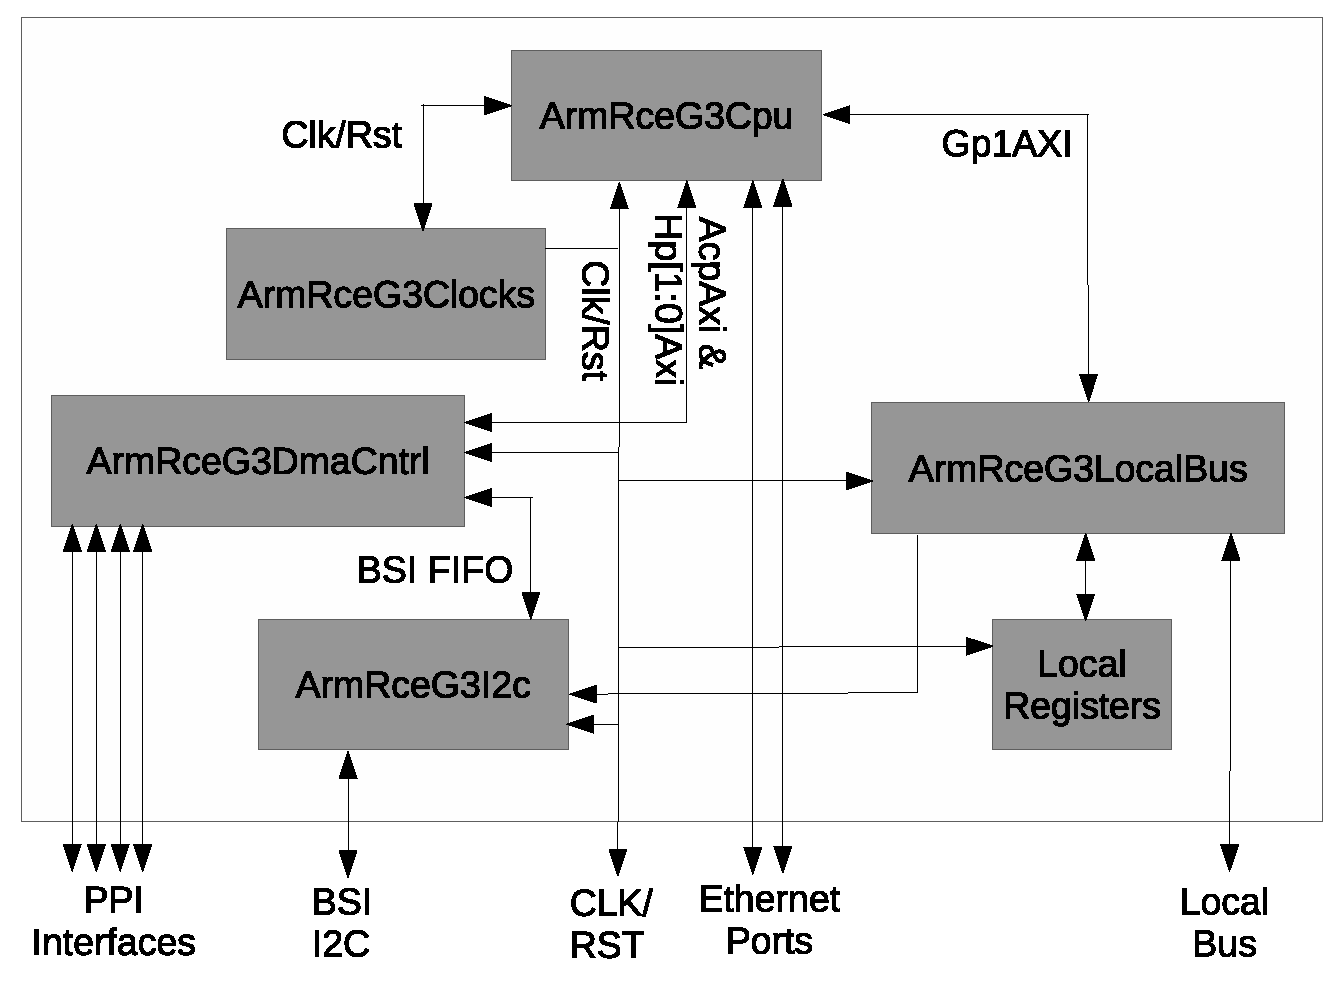
\psfig{file=images/arm_g3_top.eps,scale=0.50}
   \caption{Top Level Block Diagram}
   \label{fig:top_level_block}
\end{figure}

\subsubsection{Top Level Address Map}

The top level module contains a handful of registers as shown in the following table. 

The Version value is unique to each target FPGA design. While the format of this version value is not defined it is typical for the upper 
12 bits to be unique for each target FPGA type while the lower 20 bits are incremented with each compile.

The ArmRceG3Version value is defined in the core module and is incremented any time any of the major functions within the core module are
modified.

The BuildString value is a 256 character NULL terminated string which contains information about the user who built the image and the 
timestamp of when the image was built. This field is automatically updated by the build script at each compile.

\begin{table}[H]
\small
\centering
   \begin{tabular}{| l | l | l | l | l | } 
      \hline \textbf{Address} & \textbf{Bits} & \textbf{Mode} & \textbf{Name} & \textbf{Description} \\
      \hline 0x80000000       & 31:0          & Read     & Version         & FPGA version value. Set in Version.vhd. \\
      \hline 0x80000004       & 31:0          & R/W      & Scratchpad      & Scratchpad register.                                 \\
      \hline 0x80000008       & 31:0          & Read     & ArmRceG3Version & ARM RCE Gen3 Module Version.                         \\
      \hline 0x80000010       & 1:0           & R/W      & ClkSel0         & Reference Clock 0 Frequency Select. \\               \\
      \hline 0x80000014       & 1:0           & R/W      & ClkSel1         & Reference Clock 1 Frequency Select. \\               \\
      \hline 0x80001000 - 0x800010FF & 31:0   & Read     & BuildString     & NULL termination build user and timestamp string.    \\
      \hline
   \end{tabular}
   \caption{Top Level Address Map}
   \label{tab:top_addr}
\end{table}

\subsection{Local Bus Controller (ArmRceG3LocalBus.vhd)}
\label{subsec:ArmRceG3LocalBus}

This module implements a bridge between the general purpose AXI master port (GP1) and a simple read/write local bus. 
Transactions on the connected AXI general purpose (GP1) interface are converted to the corresponding read or write transactions on the local bus. 
The local bus controller supports single dual word (32-bit) accesses.

\subsubsection{Local Bus Interfaces}

The generic ports for the local bus controller module are shown in table \ref{tab:lb_generics}.

\begin{table}[H]
\small
\centering
   \begin{tabular}{| l | l | l | l | }
      \hline \textbf{Value} & \textbf{Type} \textbf{Default} & \textbf{Description} \\
      \hline TPD\_G          & time    & 1 ns & Synchronous signal delay value for simulation.   \\
      \hline
   \end{tabular}
   \caption{ArmRceG3LocalBus Generics}
   \label{tab:lb_generics}
\end{table}

The signal ports for the local bus controller module are shown in table \ref{tab:lb_signals}.
Any records referenced in this table are described in detail in section \ref{sec:vhdl_records}. 

\begin{table}[H]
\small
\centering
   \begin{tabular}{| l | l | l | l | l | } 
      \hline \textbf{Signal}            & \textbf{Type} & \textbf{Width} & \textbf{Direction} & \textbf{Description} \\
      \hline axiClk                     & Logic                                                      & 1  & In       & AXI interface clock       \\
      \hline axiClkRst                  & Logic                                                      & 1  & In       & AXI interface reset       \\
      \hline axiMasterReadFromArm       & \hyperref[subsec:AxiReadMasterType]{AxiReadMasterType}     & 1  & In       & AXI bus read from ARM     \\
      \hline axiMasterReadToArm         & \hyperref[subsec:AxiReadSlaveType]{AxiReadSlaveType}       & 1  & Out      & AXI bus read to ARM       \\
      \hline axiMasterWriteFromArm      & \hyperref[subsec:AxiWriteMasterType]{AxiWriteMasterType}   & 1  & In       & AXI bus read from ARM     \\
      \hline axiMasterWriteToArm        & \hyperref[subsec:AxiWriteSlaveType]{AxiWriteSlaveType}     & 1  & Out      & AXI bus read to ARM       \\
      \hline localBusMaster             & \hyperref[subsec:LocalBusMasterType]{LocalBusMasterType} & 16 & Out      & Local bus output          \\
      \hline localBusSlave              & \hyperref[subsec:LocalBusSlaveType]{LocalBusSlaveType}   & 16 & In       & Local bus input           \\
      \hline
   \end{tabular}
   \caption{ArmRceG3LocalBus Signals}
   \label{tab:lb_signals}
\end{table}

All of the module interface signals are synchronous to the rising edge of axiClk.  The assertion of axiClkRst returns all internal signals to their default states.

\subsubsection{Local Bus Write Transactions}

When the module detects the assertion of a valid write address from the AXI master it acknowledges the write address reception, stores the presented 
address and enters the wait for data state.  When the AXI master presents the write data the state machine will register the write data, acknowledge 
the completion of the write cycle to the AXI master and present the write data on the local bus as shown in figure \ref{fig:lb_write_cycle}.

Address bits 31:30 are constants for all AXI GP1 interfaces transactions. The local bus controller will use address bits 29:26 to select one of
16 local bus interface ports. All 32-bits for the address are presented on the local bus addr vector with address bits 31:26 containing a constant
value.

The writeEnable signal is asserted for a single clock cycle coincident with the 32-bit write data. 

\begin{figure}[H]
   \centering
   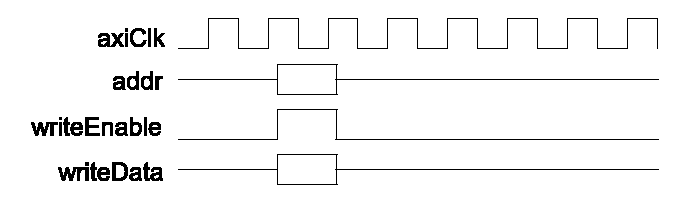
\psfig{file=images/write_cycle.eps,scale=1.0}
   \caption{Local Bus Write Cycle}
   \label{fig:lb_write_cycle}
\end{figure}

\subsubsection{Local Bus Read Transactions}

A read transaction is started by the assertion of a valid read address from the AXI master. The state machine responds to this by 
acknowledging the read address and presenting the address on the local bus. The readEnable signal is asserted to along with the 
received address on the selected local bus interface as shown in figure \ref{fig:lb_read_cycle}. 

The state machine then waits for the local bus client to return the read data on the readData vector coincident with the assertion 
of the readValid signal. The state machine will wait for up to 256 clock cycles for the local bus slave to complete the read transaction. 
If the local bus slave does not respond within this period of time the transaction will be terminated and the read data returned will be 
0xdeadbeef. Upon successful completion of a read cycle the state machine will return the read data and go back to the idle state. 

\begin{figure}[H]
   \centering
   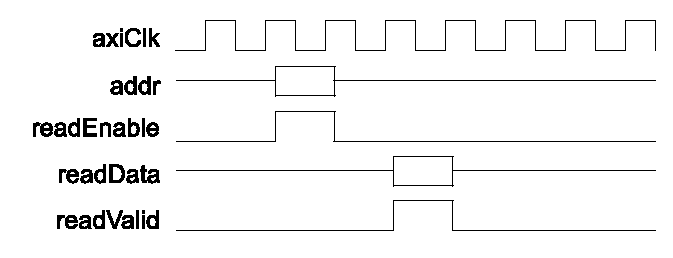
\psfig{file=images/read_cycle.eps,scale=1.0}
   \caption{Local Bus Read Cycle}
   \label{fig:lb_read_cycle}
\end{figure}

\subsubsection{Address Allocations}

The address range and channel assignments for the local bus module are show in table \ref{tab:lb_addr_ports}. 

\begin{table}[H]
\small
\centering
   \begin{tabular}{| l | l | l | } 
      \hline \textbf{Port} & \textbf{Address Range} & \textbf{Assignment} \\
      \hline Channel 0  & 0x8000\_0000 - 0x83FF\_FFFF & Top Level Registers \\
      \hline Channel 1  & 0x8400\_0000 - 0x87FF\_FFFF & BSI I2C Slave Registers \\
      \hline Channel 2  & 0x8800\_0000 - 0x8BFF\_FFFF & DMA Controller Registers \& FIFOs \\
      \hline Channel 3  & 0x8C00\_0000 - 0x8FFF\_FFFF & Unused \\
      \hline Channel 4  & 0x9000\_0000 - 0x83FF\_FFFF & Unused \\
      \hline Channel 5  & 0x9400\_0000 - 0x87FF\_FFFF & Unused \\
      \hline Channel 6  & 0x9800\_0000 - 0x8BFF\_FFFF & Unused \\
      \hline Channel 7  & 0x9C00\_0000 - 0x8FFF\_FFFF & Unused \\
      \hline Channel 8  & 0xA000\_0000 - 0xA3FF\_FFFF & External Register Space \\
      \hline Channel 9  & 0xA400\_0000 - 0xA7FF\_FFFF & External Register Space \\
      \hline Channel 10 & 0xA800\_0000 - 0xABFF\_FFFF & External Register Space \\
      \hline Channel 11 & 0xAC00\_0000 - 0xAFFF\_FFFF & External Register Space \\
      \hline Channel 12 & 0xB000\_0000 - 0xB3FF\_FFFF & External Register Space \\
      \hline Channel 13 & 0xB400\_0000 - 0xB7FF\_FFFF & External Register Space \\
      \hline Channel 14 & 0xB800\_0000 - 0xBBFF\_FFFF & External Register Space \\
      \hline Channel 15 & 0xBC00\_0000 - 0xBFFF\_FFFF & External Register Space \\
      \hline
   \end{tabular}
   \caption{Local Bus Address Space }
   \label{tab:lb_addr_ports}
\end{table}

\subsection{Clock Generation Module (ArmRceG3Clocks.vhd)}
\label{subsec:ArmRceG3Clocks}

The clock generation module generates the set of clocks required both internal and external to
the ARM RCE Gen 3 Core module. The clocks in this module can be derived from any of the four function 
clock outputs from the processor core. Currently all clocks are derived from function clock 0 which is
required to be configured as 100Mhz.

\subsubsection{Clock Generation Interfaces}

The generic ports for the clock generation module are shown in table \ref{tab:clk_gen_generics}.

\begin{table}[H]
\small
\centering
   \begin{tabular}{| l | l | l | l | }
      \hline \textbf{Value} & \textbf{Type} & \textbf{Default} & \textbf{Description} \\
      \hline TPD\_G          & time    & 1 ns & Synchronous signal delay value for simulation.   \\
      \hline AXI\_CLKDIV\_G  & real    & 4.7   & AXI bus clock divider. Clock rate = 1000Mhz / value. \\
                             &         &       & Target clock rate is 212Mhz.                         \\
      \hline
   \end{tabular}
   \caption{ArmRceG3Clocks Generics}
   \label{tab:clk_gen_generics}
\end{table}

The signal ports for the clock generation module are shown in table \ref{tab:clk_gen_signals}.
Any records referenced in this table are described in detail in section \ref{sec:vhdl_records}. 

\begin{table}[H]
\small
\centering
   \begin{tabular}{| l | l | l | l | l | } 
      \hline \textbf{Signal}            & \textbf{Type} & \textbf{Width} & \textbf{Direction} & \textbf{Description} \\
      \hline fclkClk3          & Logic   & 1  & In       & CPU function clock output 3        \\
      \hline fclkClk2          & Logic   & 1  & In       & CPU function clock output 2        \\
      \hline fclkClk1          & Logic   & 1  & In       & CPU function clock output 1        \\
      \hline fclkClk0          & Logic   & 1  & In       & CPU function clock output 0        \\
      \hline fclkRst3          & Logic   & 1  & In       & CPU function clock reset 3         \\
      \hline fclkRst2          & Logic   & 1  & In       & CPU function clock reset 2         \\
      \hline fclkRst1          & Logic   & 1  & In       & CPU function clock reset 1         \\
      \hline fclkRst0          & Logic   & 1  & In       & CPU function clock reset 0, 100Mhz \\
      \hline axiGpMasterReset  & Logic   & 2  & In       & GP master port resets              \\
      \hline axiGpSlaveReset   & Logic   & 2  & In       & GP slave port resets               \\
      \hline axiAcpSlaveReset  & Logic   & 1  & In       & ACP slave port reset               \\
      \hline axiHpSlaveReset   & Logic   & 4  & In       & HP slave port resets               \\
      \hline axiClk            & Logic   & 1  & Out      & AXI bus clock output               \\
      \hline axiClkRst         & Logic   & 1  & Out      & AXI bus clock reset                \\
      \hline sysClk125         & Logic   & 1  & Out      & System 125Mhz clock                \\
      \hline sysClk125Rst      & Logic   & 1  & Out      & System 125Mhz clock reset          \\
      \hline sysClk200         & Logic   & 1  & Out      & System 200Mhz clock                \\
      \hline sysClk200Rst      & Logic   & 1  & Out      & System 200Mhz clock reset          \\
      \hline
   \end{tabular}
   \caption{ArmRceG3Clocks Signals}
   \label{tab:clk_gen_signals}
\end{table}

\subsection{DMA Controller (ArmRceG3DmaCntrl.vhd)}
\label{subsec:ArmRceG3DmaCntrl}

The DMA controller module is a container for the logic modules which implement the protocol plug in (PPI) interfaces as well
as the BSI management interface. 

The external interfaces to this module include the 4 HP AXI processor busses, the ACP AXI processor bus, 
a portion of the local bus (see \hyperref[subsec:ArmRceG3LocalBus]{Local Bus Controller, section \ref*{subsec:ArmRceG3LocalBus}}), 
the 4 protocol plug in (PPI) interfaces, 16 processor interrupts and the I2C BSI data 
(see \hyperref[subsec:ArmRceG3I2c]{I2C Controller, section \ref*{subsec:ArmRceG3I2c}}).  

\subsubsection{DMA Controller Interfaces}

The generic ports for the DMA controller module are shown in table \ref{tab:dma_cntrl_generics}.

\begin{table}[H]
\small
\centering
   \begin{tabular}{| l | l | l | l | }
      \hline \textbf{Value} & \textbf{Type} \textbf{Default} & \textbf{Description} \\
      \hline TPD\_G          & time     & 1 ns & Synchronous signal delay value for simulation.   \\
      \hline
   \end{tabular}
   \caption{ArmRceG3DmaCntrl Generics}
   \label{tab:dma_cntrl_generics}
\end{table}

The signal ports for the DMA controller module are shown in table \ref{tab:dma_cntrl_signals}. 
Any records referenced in this table are described in detail in section \ref{sec:vhdl_records}. 

\begin{table}[H]
\small
\centering
   \begin{tabular}{| l | l | l | l | l | } 
      \hline \textbf{Signal}            & \textbf{Type} & \textbf{Width} & \textbf{Direction} & \textbf{Description} \\
      \hline axiClk                     & Logic                                                            & 1  & In       & AXI interface clock       \\
      \hline axiClkRst                  & Logic                                                            & 1  & In       & AXI interface reset       \\
      \hline axiAcpSlaveWriteFromArm  & \hyperref[subsec:AxiWriteSlaveType]{AxiWriteSlaveType}         & 1  & In       & AXI ACP bus write from ARM     \\
      \hline axiAcpSlaveWriteToArm    & \hyperref[subsec:AxiWriteMasterType]{AxiWriteMasterType}       & 1  & Out      & AXI ACP bus write to ARM       \\
      \hline axiAcpSlaveReadFromArm   & \hyperref[subsec:AxiReadSlaveType]{AxiReadSlaveType}           & 1  & In       & AXI ACP bus write from ARM     \\
      \hline axiAcpSlaveReadToArm     & \hyperref[subsec:AxiReadMasterType]{AxiReadMasterType}         & 1  & Out      & AXI ACP bus write to ARM       \\
      \hline axiHpSlaveWriteFromArm   & \hyperref[subsec:AxiWriteSlaveType]{AxiWriteSlaveType}       & 4  & In       & AXI HP bus write from ARM     \\
      \hline axiHpSlaveWriteToArm     & \hyperref[subsec:AxiWriteMasterType]{AxiWriteMasterType}     & 4  & Out      & AXI HP bus write to ARM       \\
      \hline axiHpSlaveReadFromArm    & \hyperref[subsec:AxiReadSlaveType]{AxiReadSlaveType}         & 4  & In       & AXI HP bus write from ARM     \\
      \hline axiHpSlaveReadToArm      & \hyperref[subsec:AxiReadMasterType]{AxiReadMasterType}       & 4  & Out      & AXI HP bus write to ARM       \\
      \hline interrupt         & Logic                                                        & 16 & Out      & Interrupt outputs \\
      \hline localBusMaster    & \hyperref[subsec:LocalBusMasterType]{LocalBusMasterType}     & 1  & In       & Local bus input           \\
      \hline localBusSlave     & \hyperref[subsec:LocalBusSlaveType]{LocalBusSlaveType}       & 1  & Out      & Local bus output          \\
      \hline obPpiClk          & Logic                                                        & 4  & In       & Outbound PPI clocks  \\
      \hline obPpiToFifo       & \hyperref[subsec:ObPpiToFifoType]{ObPpiToFifoType}         & 4  & In       & Outbound PPI input signals \\
      \hline obPpiFromFifo     & \hyperref[subsec:ObPpiFromFifoType]{ObPpiFromFifoType}     & 4  & Out      & Outbound PPI outout signals \\
      \hline ibPpiClk          & Logic                                                        & 4  & In       & Outbound PPI clocks  \\
      \hline ibPpiToFifo       & \hyperref[subsec:IbPpiToFifoType]{IbPpiToFifoType}         & 4  & In       & Inbound PPI input signals \\
      \hline ibPpiFromFifo     & \hyperref[subsec:IbPpiFromFifoType]{IbPpiFromFifoType}     & 4  & Out      & Inbound PPI outout signals \\
      \hline bsiToFifo         & \hyperref[subsec:QWordToFifoType]{QWordToFifoType}           & 1  & In       & BSI FIFO input signals  \\
      \hline bsiFromFifo       & \hyperref[subsec:QWordFromFifoType]{QWordFromFifoType}       & 1  & Out      & BSI FIFO output signals \\
      \hline
   \end{tabular}
   \caption{ArmRceG3DmaCntrl Signals}
   \label{tab:dma_cntrl_signals}
\end{table}

\subsubsection{DMA Controller Block Diagram}

The block diagram of the DMA controller module is shown in figure \ref{fig:dma_cntrl_block}. The following sub modules
exist within the module and are described in greater detail later in this document:

\begin{itemize}
   \item ArmRceG3IbCntrl: Container for inbound FIFO logic modules (section \ref{subsec:ArmRceG3IbCntrl})
   \item ArmRceG3IbPpi: Inbound PPI controller module (section \ref{subsec:ArmRceG3IbPpi})
   \item ArmRceG3ObCntrl: Container for outbound FIFO logic modules (section \ref{subsec:ArmRceG3ObCntrl})
   \item ArmRceG3ObPpi: Outbound PPI controller module (section \ref{subsec:ArmRceG3ObPpi})
   \item ArmRceG3DmaComp: DMA completion FIFO container module (section \ref{subsec:ArmRceG3DmaComp})
\end{itemize}

The DMA controller module also contains a number of local configuration and status registers. 

\begin{figure}[H]
   \centering
   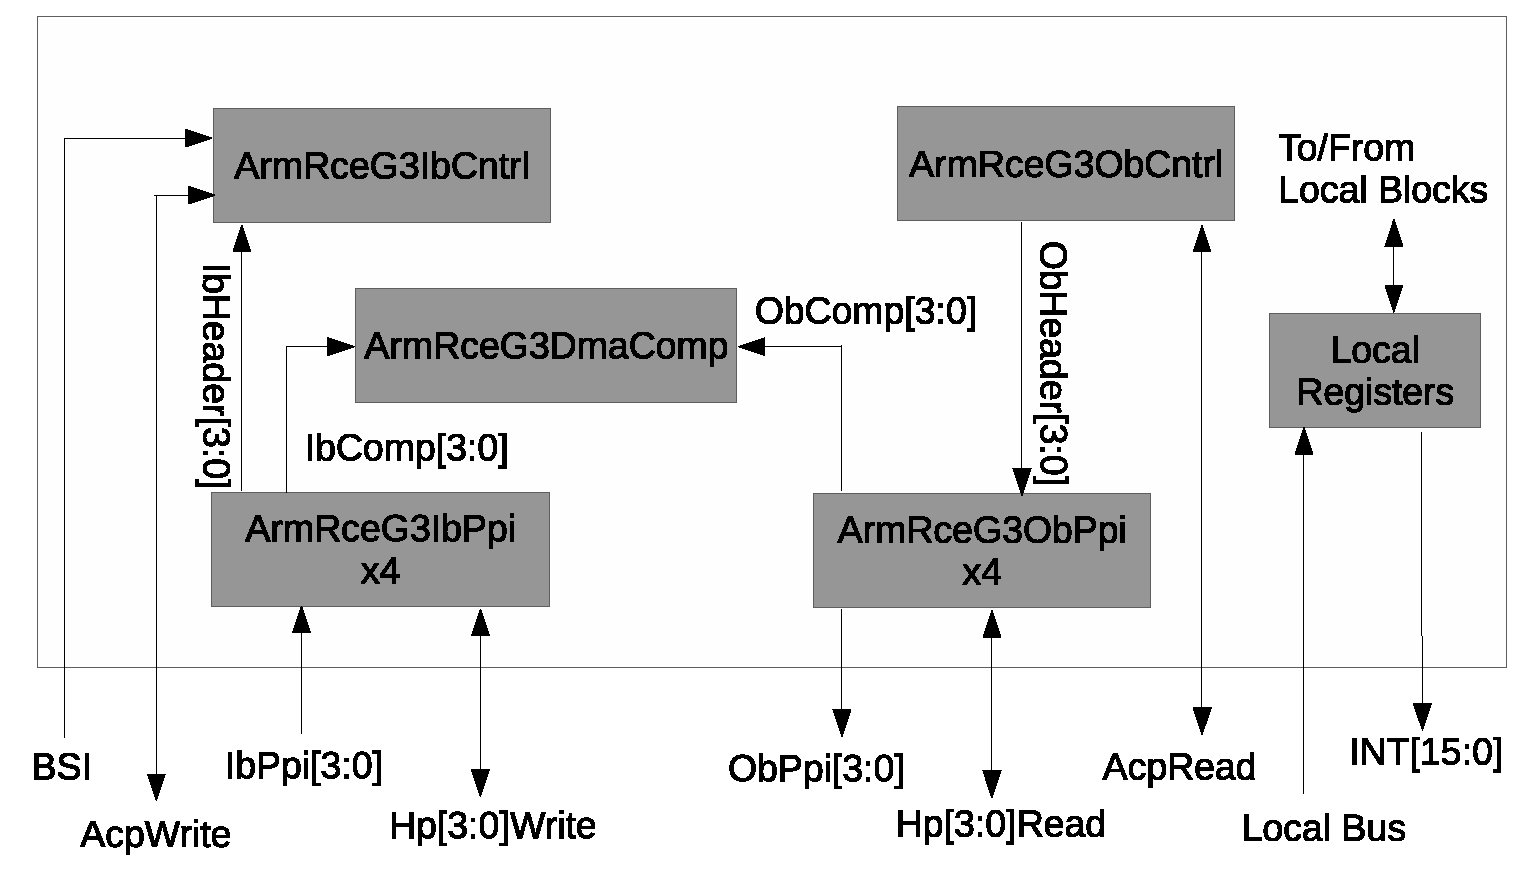
\psfig{file=images/arm_g3_dma_cntrl.eps,scale=0.50}
   \caption{DMA Controller Block Diagram}
   \label{fig:dma_cntrl_block}
\end{figure}

\subsubsection{DMA Controller Address Map}
The DMA controller module contains the register read/write logic for all of it's sub modueles. The resulting address map is shown below.

\begin{center}[H]
\small
   \begin{longtable}{| l | l | l | l | l | }
      \hline \textbf{Address} & \textbf{Bits} & \textbf{Mode} & \textbf{Name}   & \textbf{Description} \\
      \hline
      \endfirsthead
      \multicolumn{5}{c}%
      {\textit{Continued from previous page}} \\
      \hline \textbf{Address} & \textbf{Bits} & \textbf{Mode} & \textbf{Name}   & \textbf{Description} \\
      \hline
      \endhead
      \hline \multicolumn{5}{r}{\textit{Continued on next page}} \\
      \endfoot
      \hline
      \caption{DMA Controller Address Map} \\
      \endlastfoot
             0x88000000              & 31:0  & Read  & CompFifo0            & Completion FIFO 0                              \\
      \hline 0x88000004              & 31:0  & Read  & CompFifo1            & Completion FIFO 1                              \\
             \ldots                  &       &            &                      &                                                \\
      \hline 0x88000028              & 31:0  & Read  & CompFifo10           & Completion FIFO 10                             \\
      \hline 0x8800002C - 0x8800003C & NA    & Read  & Unused               & Read as zero                                   \\
      \hline 0x88000040              & 31:0  & Read  & OutboundHeader0Free  & Outbound Header 0 Free List                    \\
      \hline 0x88000044              & 31:0  & Read  & OutboundHeader1Free  & Outbound Header 1 Free List                    \\
      \hline 0x88000048              & 31:0  & Read  & OutboundHeader2Free  & Outbound Header 2 Free List                    \\
      \hline 0x8800004C              & 31:0  & Read  & OutboundHeader3Free  & Outbound Header 3 Free List                    \\
      \hline 0x88000050 - 0x880000FC & NA    & Read  & Unused               & Read as zero                                   \\
      \hline 0x88000100 - 0x8800013C & 31:0  & Write & InboundHeader0Free   & Inbound header 0, free list FIFO               \\
                                     &       &       &                      & FIFO bits 35:32 = Address bits 5:2             \\
      \hline 0x88000140 - 0x8800017C & 31:0  & Write & InboundHeader1Free   & Inbound header 1, free list FIFO               \\
                                     &       &       &                      & FIFO bits 35:32 = Address bits 5:2             \\
      \hline 0x88000180 - 0x880001BC & 31:0  & Write & InboundHeader2Free   & Inbound header 2, free list FIFO               \\
                                     &       &       &                      & FIFO bits 35:32 = Address bits 5:2             \\
      \hline 0x880001C0 - 0x880001FC & 31:0  & Write & InboundHeader3Free   & Inbound header 3, free list FIFO               \\
                                     &       &       &                      & FIFO bits 35:32 = Address bits 5:2             \\
      \hline 0x88000200 - 0x8800023C & 31:0  & Write & OutboundHeader0Tx    & Outbound header 0, transmit FIFO               \\
                                     &       &       &                      & FIFO bits 35:32 = Address bits 5:2             \\
      \hline 0x88000240 - 0x8800027C & 31:0  & Write & OutboundHeader1Tx    & Outbound header 1, transmit FIFO               \\
                                     &       &       &                      & FIFO bits 35:32 = Address bits 5:2             \\
      \hline 0x88000280 - 0x880002BC & 31:0  & Write & OutboundHeader2Tx    & Outbound header 2, transmit FIFO               \\
                                     &       &       &                      & FIFO bits 35:32 = Address bits 5:2             \\
      \hline 0x880002C0 - 0x880002FC & 31:0  & Write & OutboundHeader3Tx    & Outbound header 3, transmit FIFO               \\
                                     &       &       &                      & FIFO bits 35:32 = Address bits 5:2             \\
      \hline 0x88000300              & NA    & Write & MemChan0DirtyClear   & Write to clear memory channel 0                \\
      \hline 0x88000304              & NA    & Write & MemChan1DirtyClear   & Write to clear memory channel 1                \\
             \ldots                  &       &       &                      &                                                \\
      \hline 0x88000310              & NA    & Write & MemChan4DirtyClear   & Write to clear memory channel 4                \\
      \hline 0x88000314 - 0x880003FC & NA    & Read  & Unused               & Read as zero                                   \\
      \hline 0x88000400              & 3:0   & Read  & IbDirtyStatus        & Inbound memory dirty, one bit per channel \\
                                     & 4     & Read  & BsiDirtyStatus       & BSI memory dirty, one bit per channel \\
                                     & 15:5  & Read  & CompFifoStatus       & Completion FIFO ready, one bit per channel \\
      \hline 0x88000404              & 15:0  & R/W   & InterruptEnable      & Interrupt enable, one bit per interrupt        \\
      \hline 0x88000408              & 3:0   & R/W   & HeaderWriteDmaCache  & Header AXI write cache configuration           \\
      \hline 0x8800040C              & 3:0   & R/W   & HeaderReadDmaCache   & Header AXI read cache configuration            \\
      \hline 0x88000410              & 3:0   & R/W   & IbFifoEnable         & Inbound header enables                         \\
                                     & 4     & R/W   & BsiFifoEnable        & BSI FIFO enable                                \\
                                     & 8:5   & R/W   & ObFifoEnable         & Outbound header enables                        \\
      \hline 0x88000418              & 31:18 & R/W   & MemBaseAddress       & Memory base address                            \\
      \hline 0x8800041C              & 3:0   & R/W   & PpiReadDmaCache      & PPI AXI read cache configuration               \\
      \hline 0x88000420              & 3:0   & R/W   & PpiWriteDmaCache     & PPI AXI write cache configuration              \\
      \hline 0x88000424              & 3:0   & R/W   & PpiIbOnline[3:0]     & Inbound PPI online configuration              \\
                                     & 7:4   & R/W   & PpiObOnline[3:0]     & Outbound PPI online configuration             \\
      \hline 0x88000428 - 0x880004FC & NA    & Read  & Unused               & Read as zero                                   \\
      \hline 0x88000500 - 0x8800053C & 31:0  & Write & InboundPpi0Control   & Inbound PPI 0 Control FIFO                     \\
                                     &       &       &                      & FIFO bits 35:32 = Address bits 5:2             \\
      \hline 0x88000540 - 0x8800057C & 31:0  & Write & InboundPpi1Control   & Inbound PPI 1 Control FIFO                     \\
                                     &       &       &                      & FIFO bits 35:32 = Address bits 5:2             \\
      \hline 0x88000580 - 0x880005BC & 31:0  & Write & InboundPpi2Control   & Inbound PPI 2 Control FIFO                     \\
                                     &       &       &                      & FIFO bits 35:32 = Address bits 5:2             \\
      \hline 0x880005C0 - 0x880005FC & 31:0  & Write & InboundPpi3Control   & Inbound PPI 3 Control FIFO                     \\
                                     &       &       &                      & FIFO bits 35:32 = Address bits 5:2             \\
      \hline 0x88000600              & 31:0  & Read  & IbPpi0Id             & Inbound PPI 0 ID value                         \\
      \hline 0x88000604              & 31:0  & Read  & IbPpi0Id             & Inbound PPI 0 version value                      \\
      \hline 0x88000608              & 31:0  & Read  & IbPpi0ConfigA        & Inbound PPI 0 config word A              \\
      \hline 0x8800060C              & 31:0  & Read  & IbPpi0ConfigB        & Inbound PPI 0 config word B              \\
             \ldots                  &       &       &                      &                                                \\
      \hline 0x88000630              & 31:0  & Read  & IbPpi3Id             & Inbound PPI 3 ID value                         \\
      \hline 0x88000634              & 31:0  & Read  & IbPpi3Id             & Inbound PPI 3 version value                      \\
      \hline 0x88000638              & 31:0  & Read  & IbPpi3ConfigA        & Inbound PPI 3 config word A              \\
      \hline 0x8800063C              & 31:0  & Read  & IbPpi3ConfigB        & Inbound PPI 3 config word B              \\
      \hline 0x88000640              & 31:0  & Read  & ObPpi0Id             & Outbound PPI 0 ID value                         \\
      \hline 0x88000644              & 31:0  & Read  & ObPpi0Id             & Outbound PPI 0 version value                      \\
      \hline 0x88000648              & 31:0  & Read  & ObPpi0ConfigA        & Outbound PPI 0 config word A              \\
      \hline 0x8800064C              & 31:0  & Read  & ObPpi0ConfigB        & Outbound PPI 0 config word B              \\
             \ldots                  &       &       &                      &                                                \\
      \hline 0x88000670              & 31:0  & Read  & ObPpi3Id             & Outbound PPI 3 ID value                         \\
      \hline 0x88000674              & 31:0  & Read  & ObPpi3Id             & Outbound PPI 3 version value                      \\
      \hline 0x88000678              & 31:0  & Read  & ObPpi3ConfigA        & Outbound PPI 3 config word A              \\
      \hline 0x8800067C              & 31:0  & Read  & ObPpi3ConfigB        & Outbound PPI 3 config word B              \\
      \hline
   \end{longtable}
   \label{tab:dma_addr}
\end{center}

A number of FIFOs in the above table are 36-bit FIFOs which are written to over the 32-bit local bus. The upper 4 bits of the FIFO are derived by 
the offset address used when writing to the FIFO. The address for the FIFO write can be derived using the following
equation:

\begin{center}
Address = (FIFO base address) * 4 * (Bits 35:32)
\end{center}

For example to write the value 0xA\_5A5A\_5A5A to the Inbound header 0 free list FIFO, one 
would write the 32-bit value 0x5A5A\_5A5A to the address 0x8800\_0128.

\subsubsection{DMA Controller Interrupt Mapping}

The DMA controller supports 16 interrupt putputs, each with it's own enable bit. The sources of these 16 interrupts are described in the table below.

\begin{table}[H]
\small
\centering
   \begin{tabular}{| l | l | l | }
      \hline \textbf{Interrupt} & \textbf{Name}  & \textbf{Description} \\
      \hline 3:0            & IbDesc[3:0]    &  Inbound header 3:0 descriptor FIFOs. \\
                            &                &  Asserted when associated quad word memory location \\
                            &                &  is dirty. De-asserted when the associated memory location \\
                            &                &  is cleaned by writing to corresponding dirty clear address. \\
      \hline 4              & BsiData        &  BSI data FIFO.                      \\
                            &                &  Asserted when associated quad word memory location \\
                            &                &  is dirty. De-asserted when the associated memory location \\
                            &                &  is cleaned by writing to corresponding dirty clear address. \\
      \hline 15:5           & CompFifo[10:0] &  Completion FIFOs.                   \\
                            &                &  Asserted when associated completion FIFO has at least one entry. \\
                            &                &  De-asserted when the associated completion FIFO is empty. \\
      \hline
   \end{tabular}
   \caption{DMA Controller Interrupt Mapping}
   \label{tab:dma_int_mappings}
\end{table}

\subsection{Inbound Controller (ArmRceG3IbCntrl.vhd)}
\label{subsec:ArmRceG3IbCntrl}

The inbound controller module is a sub-container within the DMA controller which contains the logic to support inbound PPI traffic. 
This includes the 4 inbound header engines, the 5 quad word FIFOs, the memory space dirty state tracking logic and an AXI write controller.
The AXI write controller is the interface between the various write engines and the write interface of the AXI ACP processor bus. 

\subsubsection{Inbound Controller Interfaces}

The generic ports for the inbound controller module are shown in table \ref{tab:ib_cntrl_generics}.

\begin{table}[H]
\small
\centering
   \begin{tabular}{| l | l | l | l | }
      \hline \textbf{Value} & \textbf{Type} \textbf{Default} & \textbf{Description} \\
      \hline TPD\_G          & time     & 1 ns & Synchronous signal delay value for simulation.   \\
      \hline
   \end{tabular}
   \caption{ArmRceG3IbCntrl Generics}
   \label{tab:ib_cntrl_generics}
\end{table}

The signal ports for the inbound controller module are shown in table \ref{tab:ib_cntrl_signals}.
Any records referenced in this table are described in detail in section \ref{sec:vhdl_records}. 

\begin{table}[H]
\small
\centering
   \begin{tabular}{| l | l | l | l | l | } 
      \hline \textbf{Signal}            & \textbf{Type} & \textbf{Width} & \textbf{Direction} & \textbf{Description} \\
      \hline axiClk                     & Logic                                                            & 1  & In       & AXI interface clock       \\
      \hline axiClkRst                  & Logic                                                            & 1  & In       & AXI interface reset       \\
      \hline axiAcpSlaveWriteFromArm    & \hyperref[subsec:AxiWriteSlaveType]{AxiWriteSlaveType}         & 1  & In       & AXI ACP bus write from ARM \\
      \hline axiAcpSlaveWriteToArm      & \hyperref[subsec:AxiWriteMasterType]{AxiWriteMasterType}       & 1  & Out      & AXI ACP bus write to ARM  \\
      \hline dirtyFlag                  & Logic                                                        & 5  & Out      & Dirty flag vector \\
      \hline dirtyFlagClrEn             & Logic                                                        & 1  & In       & Dirty flag clear enable \\
      \hline dirtyFlagClrSel            & Logic                                                        & 4  & In       & Dirty flag clear select \\
      \hline headerPtrWrite             & Logic                                                        & 4  & In       & Header pointer write enable \\
      \hline headerPtrData              & Logic                                                        & 36 & In       & Header pointer write data \\
      \hline fifoEnable                 & Logic                                                        & 5  & In       & FIFO enable control \\
      \hline memBaseAddress             & Logic                                                        & 14 & In       & Memory base address \\
      \hline writeDmaCache              & Logic                                                        & 4 & In        & Write DMA cache configuration \\
      \hline ibHeaderClk                & Logic                                                        & 4 & In        & Inbound header FIFO clock     \\
      \hline ibHeaderToFifo             & \hyperref[subsec:IbHeaderToFifoType]{IbHeaderToFifoType}   & 4 & In        & Inbound header FIFO inputs    \\
      \hline ibHeaderFromFifo           & \hyperref[subsec:IbHeaderFromFifoType]{IbHeaderFromFifoType} & 4 & Out      & Inbound header FIFO outputs   \\
      \hline qwordToFifo                & \hyperref[subsec:QWordToFifoType]{QWordToFifoType}         & 1   & In       & BSI Quad word FIFO input signals  \\
      \hline qwordFromFifo              & \hyperref[subsec:QWordFromFifoType]{QWordFromFifoType}     & 1   & Out      & BSI Quad word FIFO output signals \\
      \hline
   \end{tabular}
   \caption{ArmRceG3IbCntrl Signals}
   \label{tab:ib_cntrl_signals}
\end{table}

A number of configuration values are included in the above interface list. The register configurable memBaseAddress vector is used as the upper 
14 bits (31:18) of the inbound header data DMA transfers as well as the base address for the quad word FIFO memory space. The writeDmaCache vector
is used as the value in the awcache field of the ACP processor bus interface during write transactions.

\subsubsection{Inbound Controller Block Diagram}

The block diagram of the inbound controller module is shown in figure \ref{fig:ib_cntrl_block}. The following sub modules
exist within the module and are described in greater detail later in this document:

\begin{itemize}
   \item ArmRceG3IbHeaderFifo: Inbound header transfer FIFO and control logic (section \ref{subsec:ArmRceG3IbHeaderFifo})
   \item ArmRceG3IbQWordFifo: Inbound Quad Word FIFO and control logic (section \ref{subsec:ArmRceG3IbQWordFifo})
   \item ArmRceG3AxiWriteCntrl: AXI write controller (section \ref{subsec:ArmRceG3AxiWriteCntrl})
\end{itemize}

The inbound controller module also contains dirty status logic which tracks the state of the OCM memory locations associated
with the 5 quad word FIFO modules.


\begin{figure}[H]
   \centering
   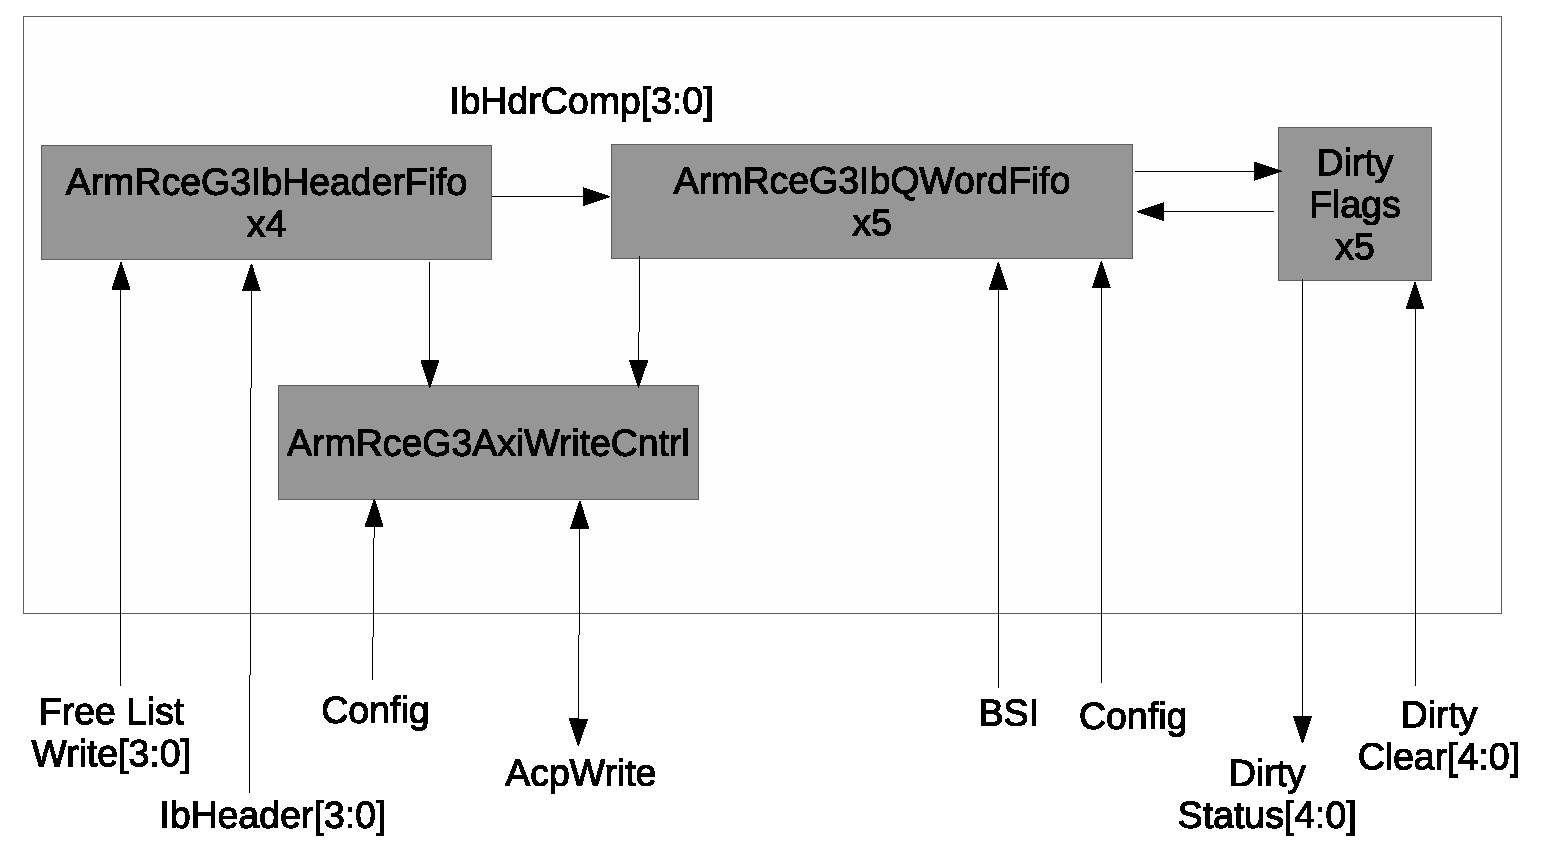
\psfig{file=images/arm_g3_ib_cntrl.eps,scale=0.50}
   \caption{Inbound Controller Block Diagram}
   \label{fig:ib_cntrl_block}
\end{figure}

\subsubsection{Quad Word FIFO Channels}

The inbound controller contains 5 instances of the Quad Word FIFO module described in section \ref{subsec:ArmRceG3IbQWordFifo}. The assignment and destination
memory address of each of these instances is shown in table \ref{tab:ib_qword_mappings}.

\begin{table}[H]
\small
\centering
   \begin{tabular}{| l | l | l | l | }
      \hline \textbf{Index} & \textbf{Name}  & \textbf{Destination Address} & \textbf{Description} \\
      \hline 0              & IbDesc0        & memBaseAddress + 0x00 &  Inbound header 0 descriptor FIFO \\
      \hline 1              & IbDesc1        & memBaseAddress + 0x08 &  Inbound header 1 descriptor FIFO \\
      \hline 2              & IbDesc2        & memBaseAddress + 0x10 &  Inbound header 2 descriptor FIFO \\
      \hline 3              & IbDesc3        & memBaseAddress + 0x18 &  Inbound header 3 descriptor FIFO \\
      \hline 4              & BsiData        & memBaseAddress + 0x20 &  BSI data FIFO                       \\
      \hline
   \end{tabular}
   \caption{Quad Word FIFO Channels}
   \label{tab:ib_qword_mappings}
\end{table}

The four inbound header descriptor FIFOs are populated when the inbound header engine (see section \ref{subsec:ArmRceG3IbHeaderFifo})
completes a header transfer. The BSI data FIFO is populated when the IPMI controller writes a 32-bit word to the
BSI shared memory over the management I2C bus (see section \ref{subsec:ArmRceG3I2c}). 

\subsubsection{ACP Write ID Mapping}

The ACP AXI interface only supports 8 independent transaction IDs. Since the inbound controller contains 5 potentional masters, some
IDs need to be shared. Table \ref{tab:ib_id_mappings} shows the allocation of AXI IDs to the masters within the inbound
controller. Only one master assigned to an ID can have an outstanding write transactions at any given time. Any other
masters which share an ID with a master who has an outstanding transaction will not attempt to access the ACP bus
until the outstanding transaction completes.

\begin{table}[H]
\small
\centering
   \begin{tabular}{| l | l | l |}
      \hline \textbf{AXI ID} & \textbf{FIFO(s)}      & \textbf{Function(s)}    \\
      \hline 0               & IbHeaderFifo0         & Inbound header 0 engine \\
      \hline 1               & IbHeaderFifo1         & Inbound header 1 engine \\
      \hline 2               & IbHeaderFifo2         & Inbound header 2 engine \\
      \hline 3               & IbHeaderFifo3         & Inbound header 3 engine \\
      \hline 4               & QWordFifo0            & Inbound header 0 descriptor FIFO    \\
                             & QWordFifo4            & BSI FIFO                \\
      \hline 5               & QWordFifo1            & Inbound header 1 descriptor FIFO   \\
      \hline 6               & QWordFifo2            & Inbound header 2 descriptor FIFO   \\
      \hline 7               & QWordFifo3            & Inbound header 3 descriptor FIFO   \\
      \hline
   \end{tabular}
   \caption{ACP Write ID Mapping}
   \label{tab:ib_id_mappings}
\end{table}

\subsection{Quad Word FIFO Controller (ArmRceG3IbQWordFifo.vhd)}
\label{subsec:ArmRceG3IbQWordFifo}

The quad word FIFO controller is a block of logic which serves as a 63-bit FIFO with direct access to the on chip memory (OCM) contained within the 
Zynq processor. Only 63 bits are available because the upper bit is used for handshaking between the quad word FIFO module and the software 
driver. 

When an entry is available in the FIFO, the transfer state machine will check to see if the associated OCM memory space
is clearn or dirty as indicated by the 5-bit dirty vector managed by the indbound controller module. If the associated memory location 
is clean the transfer state machine will pull the 63-bit value from the FIFO and write it to the associated OCM memory location. Bit 64
of the memory location will be set to zero to indicate that the location has been updated.

All transactions generated by the quad word FIFO controller are a single 64-bit write transaction on the ACP bus. Once the write data portion
of the transaction is completed the transfer state machine will release the AXI bus. The associated AXI ID will be marked busy while the state 
machine waits for the write transaction to be acknowledged by the AXI bus.  When the write has completed the transfer state machine will clear 
the ID busy signal, mark the memory location as dirty and return to the idle state. 

If enabled the dirty flag of the memory location will trigger a processor interrupt. Some time later, after accessing the associated memory location 
in OCM, software will clean the memory location by performing a write access to the associated address space. The transfer state machine will
then transfer the next FIFO entry when available.

The FIFO logic will not operated until its associated fifoEnable signal is set via register access.

\subsubsection{Quad Word FIFO Controller Interfaces}

The generic ports for the quad word FIFO controller module are shown in table \ref{tab:qword_cntrl_generics}.

\begin{table}[H]
\small
\centering
   \begin{tabular}{| l | l | l | l | }
      \hline \textbf{Value} & \textbf{Type} & \textbf{Default} & \textbf{Description} \\
      \hline TPD\_G          & time     & 1 ns & Synchronous signal delay value for simulation.    \\
      \hline MEM\_CHAN\_G    & positive & 1    & Assigned memory channel for 64-bit writes. 0 - 8. \\
      \hline
   \end{tabular}
   \caption{ArmRceG3IbQWordFifo Generics}
   \label{tab:qword_cntrl_generics}
\end{table}

The signal ports for the quad word FIFO controller module are shown in table \ref{tab:ib_cntrl_signals}.
Any records referenced in this table are described in detail in section \ref{sec:vhdl_records}. 

\begin{table}[H]
\small
\centering
   \begin{tabular}{| l | l | l | l | l | } 
      \hline \textbf{Signal}            & \textbf{Type} & \textbf{Width} & \textbf{Direction} & \textbf{Description} \\
      \hline axiClk                     & Logic                                                            & 1  & In       & AXI interface clock       \\
      \hline axiClkRst                  & Logic                                                            & 1  & In       & AXI interface reset       \\
      \hline axiWriteToCntrl            & \hyperref[subsec:AxiWriteToCntrlType]{AxiWriteToCntrlType}       & 1  & Out      & Write structure from controller \\
      \hline axiWriteFromCntrl          & \hyperref[subsec:AxiWriteFromCntrlType]{AxiWriteFromCntrlType}   & 1  & In       & Write structure to controller \\
      \hline memDirty                   & Logic                                                            & 1  & In       & Memory dirty status \\
      \hline memDirtySet                & Logic                                                            & 1  & Out      & Memory dirty status set \\
      \hline writeDmaBusyOut            & Logic                                                            & 8  & Out      & Write channel is busy output \\
      \hline writeDmaBusyIn             & Logic                                                            & 8  & In       & Write channel is busy input \\
      \hline fifoEnable                 & Logic                                                            & 1  & In       & FIFO enable control \\
      \hline writeDmaId                 & Logic                                                            & 3  & In       & Assigned write channel \\
      \hline memBaseAddress             & Logic                                                            & 14 & In       & Memory base address \\
      \hline qwordToFifo                & \hyperref[subsec:QWordToFifoType]{QWordToFifoType}               & 1  & In       & Quad word FIFO input signals  \\
      \hline qwordFromFifo              & \hyperref[subsec:QWordFromFifoType]{QWordFromFifoType}           & 1  & Out      & Quad word FIFO output signals \\
      \hline
   \end{tabular}
   \caption{ArmRceG3IbQWordFifo Signals}
   \label{tab:qword_cntrl_signals}
\end{table}

\subsubsection{Quad Word FIFO Block Diagram}

The quad word FIFO module consists of a 72-bit wide by 512 entry deep input FIFO and a transfer state machine.

\begin{figure}[H]
   \centering
   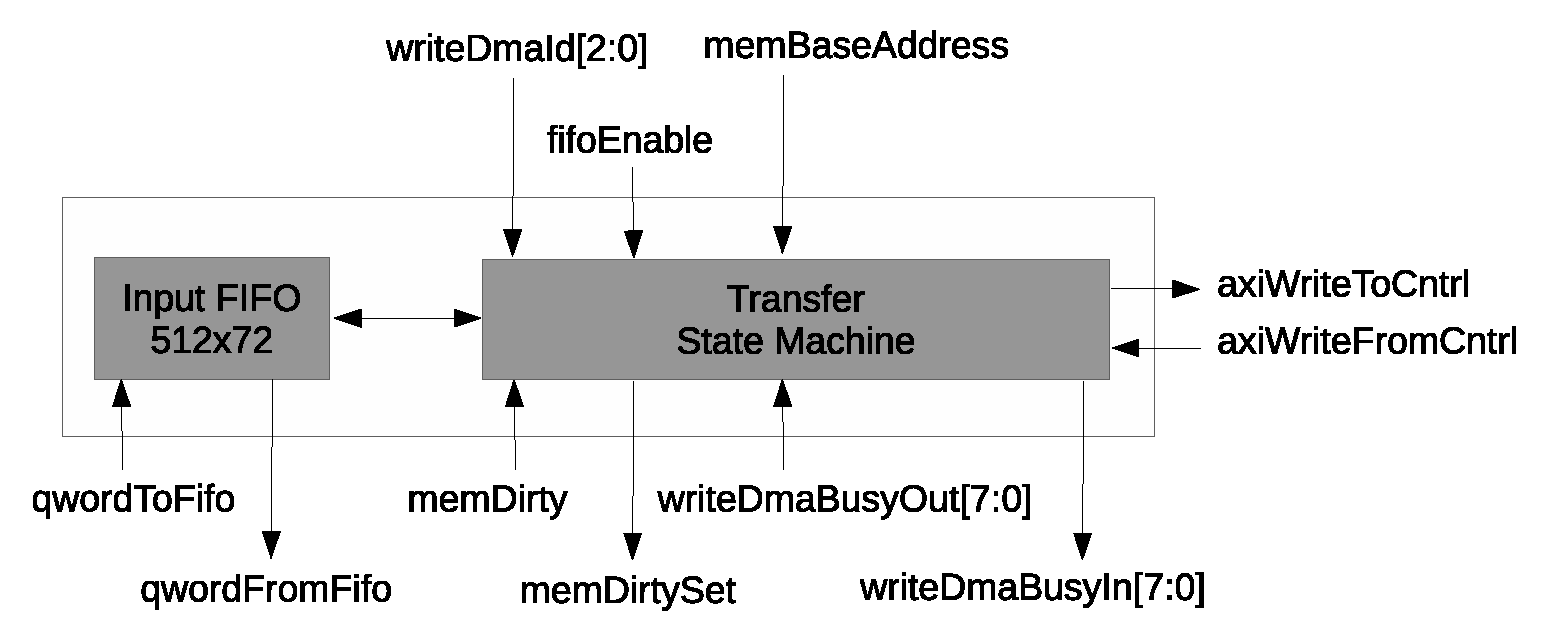
\psfig{file=images/arm_g3_qw_fifo.eps,scale=0.50}
   \caption{Quad Word FIFO Block Diagram}
   \label{fig:qw_fifo_block}
\end{figure}

\subsection{Inbound Header FIFO (ArmRceG3IbHeaderFifo.vhd)}
\label{subsec:ArmRceG3IbHeaderFifo}

The function of the inbound header FIFO module is to receive a PPI header and transfer it into on chip memory (OCM). 

When data is available in the FIFO the transfer engine will exit the idle state and pull a free descriptor entry
from the free list FIFO. The write address vector within the transfer engine is then preset with the sum of the
memBaseAddress and offset address contained in the descriptor. The offset value in the descriptor must be aligned to 
a cache line boundary.

Each AXI bus transaction originated by the transfer engine is a fixed size containing 32 bytes of data. 
The transfer engine will wait until a 32-byte block of data is ready in the FIFO or the end
of header (EOH) signal is detected. The transfer engine will request and release access to the AXI bus for each 32 byte
write transaction. If the EOH is in a position short of the 32 byte boundary, the transfer engine will continue to write
undefined data past the EOH location to the OCM.

When the entire frame has been transfered (as indicated by the EOH flag) the transfer engine will 
wait for all of the outstanding writes to complete. The transfer engine will then form a receive descriptor and 
write it to the associated inbound descriptor quad word FIFO. Along with the header length the type and mgmt flags 
from the received frame are included in the receive descriptor along with the error flag.

The inbound header FIFO will not operate if the associated fifoEnable configuration bit is not set.

\subsubsection{Inbound Header FIFO Interfaces}

The generic ports for the inbound header FIFO module are shown in table \ref{tab:ib_header_generics}.

\begin{table}[H]
\small
\centering
   \begin{tabular}{| l | l | l | l | }
      \hline \textbf{Value} & \textbf{Type} & \textbf{Default} & \textbf{Description} \\
      \hline TPD\_G          & time     & 1 ns & Synchronous signal delay value for simulation.    \\
      \hline
   \end{tabular}
   \caption{ArmRceG3IbHeaderFifo Generics}
   \label{tab:ib_header_generics}
\end{table}

The signal ports for the inbound header FIFO module are shown in table \ref{tab:ib_header_signals}.
Any records referenced in this table are described in detail in section \ref{sec:vhdl_records}. 

\begin{table}[H]
\small
\centering
   \begin{tabular}{| l | l | l | l | l | } 
      \hline \textbf{Signal}            & \textbf{Type} & \textbf{Width} & \textbf{Direction} & \textbf{Description} \\
      \hline axiClk                     & Logic                                                          & 1  & In  & AXI interface clock       \\
      \hline axiClkRst                  & Logic                                                          & 1  & In  & AXI interface reset       \\
      \hline axiWriteToCntrl            & \hyperref[subsec:AxiWriteToCntrlType]{AxiWriteToCntrlType}     & 1  & Out & Write structure to controller \\
      \hline axiWriteFromCntrl          & \hyperref[subsec:AxiWriteFromCntrlType]{AxiWriteFromCntrlType} & 1  & In  & Write structure from controller \\
      \hline headerPtrWrite             & Logic                                                          & 1  & In  & Header pointer write enable \\
      \hline headerPtrData              & Logic                                                          & 36 & In  & Header pointer write data \\
      \hline fifoEnable                 & Logic                                                          & 1  & In  & FIFO enable control \\
      \hline memBaseAddress             & Logic                                                          & 14 & In  & Memory base address \\
      \hline writeDmaId                 & Logic                                                          & 3  & In  & Write DMA ID \\
      \hline qwordToFifo                & \hyperref[subsec:QWordToFifoType]{QWordToFifoType}             & 1  & Out & Quad word FIFO output signals  \\
      \hline qwordFromFifo              & \hyperref[subsec:QWordFromFifoType]{QWordFromFifoType}         & 1  & In  & Quad word FIFO input signals \\
      \hline ibHeaderClk                & Logic                                                          & 1  & In  & Inbound header FIFO clock     \\
      \hline ibHeaderToFifo             & \hyperref[subsec:IbHeaderToFifoType]{IbHeaderToFifoType}       & 1  & In  & Inbound header FIFO input    \\
      \hline ibHeaderFromFifo           & \hyperref[subsec:IbHeaderFromFifoType]{IbHeaderFromFifoType}   & 1  & Out & Inbound header FIFO output   \\
      \hline
   \end{tabular}
   \caption{ArmRceG3IbHeaderFifo Signals}
   \label{tab:ib_header_signals}
\end{table}

\subsubsection{Inbound Header FIFO Block Diagram}

The inbound header FIFO module consists of a 72-bit wide by 512 entry deep input FIFO and a transfer state machine. A 36-bit x 512 entry FIFO is used
for the inbound free list. 

\begin{figure}[H]
   \centering
   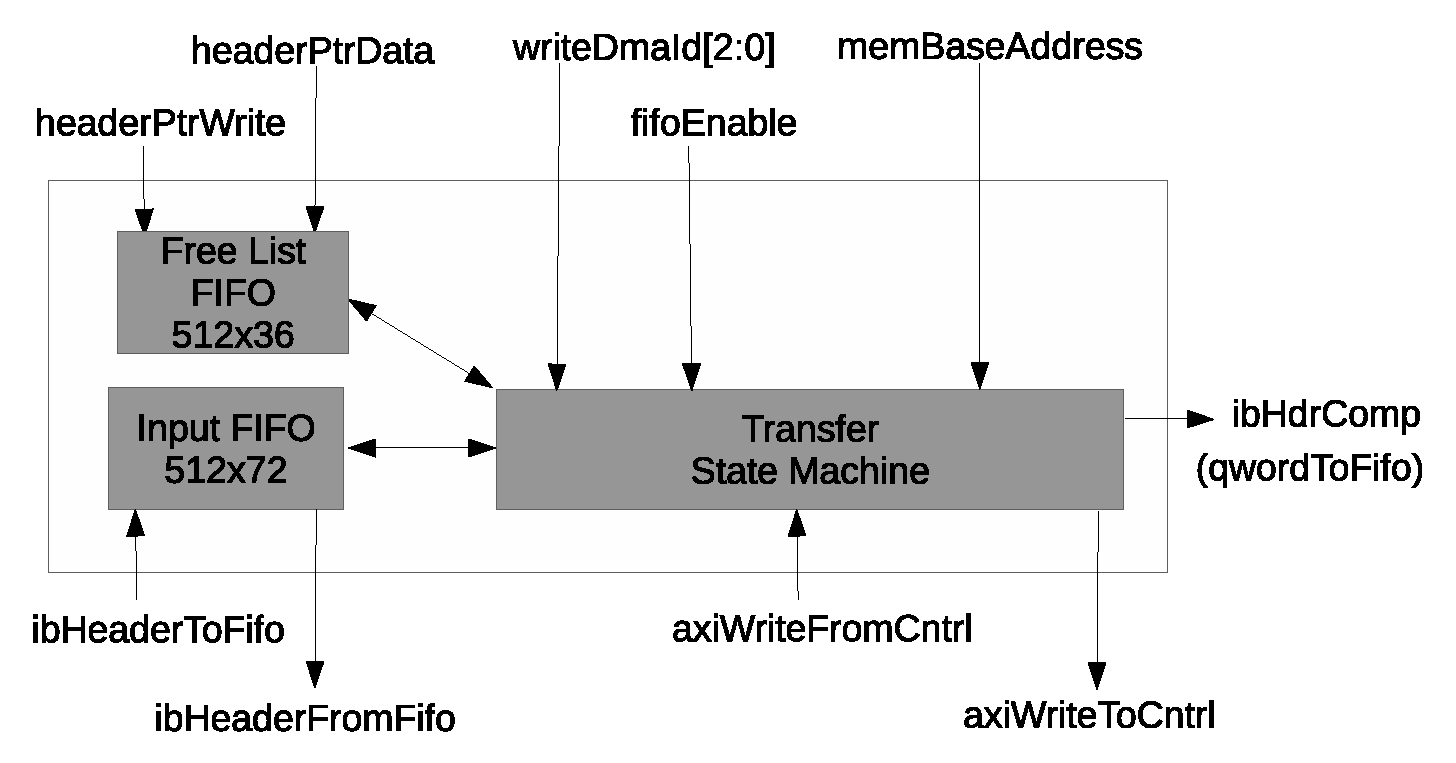
\psfig{file=images/arm_g3_ib_head_block.eps,scale=0.50}
   \caption{Inbound Header FIFO Block Diagram}
   \label{fig:ib_head_block}
\end{figure}

\subsubsection{Inbound Header Free List}

The inbound header free list contains a pool of memory address to which incoming headers are to be transfered.
This free list is populated by writing the allocated buffer address to the appropriate register address.
Since the upper data bits (35:32) of the free list FIFOs are not used only the base address for each FIFO is utilized. 
Each free list FIFO is capable of holding 511 free list entries.

The format of the receive free list entry is shown in table \ref{tab:ib_rx_flist}.

\begin{table}[H]
\small
\centering
   \begin{tabular}{| l | l | l | } 
      \hline \textbf{Bits} & \textbf{Name} & \textbf{Description} \\
      \hline 35:19         & unused        & ignored \\
      \hline 17:3          & address       & This field contains the offset address to which the inbound frame \\
                           &               & will be transfered. This address is relative to the configured base address  \\
                           &               & and must be cache line aligned.                                              \\
      \hline 2:0           & address       & Unused. The lower three address bits are assumed to be zero.               \\
      \hline
   \end{tabular}
   \caption{Inbound Header Free List Entry}
   \label{tab:ib_rx_flist}
\end{table}

\subsubsection{Inbound Header Receive Descriptor}

When an inbound header is received the inbound header logic will pull an address from the free list and DMA the header data to the associated address. 
When the operation has completed a receive descriptor will be placed in the associated receive queue. 
The receive queue is implemented in a \hyperref[subsec:ArmRceG3IbQWordFifo]{Quad Word FIFO} described in section \ref{subsec:ArmRceG3IbQWordFifo}. 
The mapping of the quad word FIFOs are described in section \ref{subsec:ArmRceG3IbCntrl}.

The format of the receive queue descriptor is shown in table \ref{tab:ib_rx_desc}.

\begin{table}[H]
\small
\centering
   \begin{tabular}{| l | l | l | } 
      \hline \textbf{Bits} & \textbf{Name} & \textbf{Description} \\
      \hline 63            & handshake     & Set to zero by firmware when valid     \\
      \hline 62:61         & unused        & Always zero                                                            \\ 
      \hline 60            & error         & This bit is set when the error bit was set on the inbound header.      \\
                           &               & This state is only possible when the inbound PPI frame has no payload. \\
      \hline 59:52         & unused        & Always zero                                                       \\
      \hline 51            & mgmt          & mgmt field from inbound frame                                          \\ 
      \hline 50:48         & htype         & frame type field from inbound frame                                    \\
      \hline 47:40         & unused        & Always zero                                                       \\
      \hline 39:32         & length        & Length of received header. One based length (1=1, 2=2)                 \\
                           &               & Specified in number of 64-bit quad words transfered.                   \\
      \hline 31:18         & unused        & Always zero                                                       \\
      \hline 17:3          & address       & This field contains the offset address to which the inbound frame \\
                           &               & was transfered. This address is relative to the configured base address \\
                           &               & and must be cache line aligned.                                         \\
      \hline 2:0           & address       & These bits are always zero.                                                \\
      \hline
   \end{tabular}
   \caption{Inbound Header Receive Descriptor}
   \label{tab:ib_rx_desc}
\end{table}

\subsubsection{Inbound Header Flow Control}

The inbound header module asserts three flow control signals depending on the state of the input FIFO:

\begin{itemize}
  \item Full           = The FIFO is full, no free entries available.
  \item Almost Full    = The FIFO is almost full with one free entry left.
  \item Partially Full = The FIFO has less than 255 entries (out of 512) available.
\end{itemize}

\subsection{Inbound PPI Controller (ArmRceG3IbPpi.vhd)}
\label{subsec:ArmRceG3IbPpi}

The inbound PPI controller receives a complete PPI frame and separates the header from the payload. The header portion of the frame is forwarded  
to the associated inbound header controller module. Meanwhile payload portion of the frame is stored in a local FIFO. The internal state machine will
wait until a inbound PPI descriptor is available in the PPI control FIFO. This descriptor described in table \ref{tab:ib_ppi_cntrl} contains
the information needed to transfer the PPI frame into processor memory. When the inbound DMA operation has completed, a completion descriptor
is written to a targeted completion FIFO. The contents of this completion descriptor are detailed in table \ref{tab:ib_ppi_comp}.

Each inbound PPI engine is attached to one of the four HP AXI write interfaces. This dedicated connection means that the inbound PPI engine
can assume complete ownership of the interface. A simplified version of the AXI write controller (described in section \ref{subsec:ArmRceG3AxiWriteCntrl})
is instantiated in the module in order to simplify the state machine and improve timing performance. In order to ensure AXI bus efficiency all write 
transfers are a fixed size of 128 bytes. The write enable strobes are used to insure that only relevant payload data is written to memory and that the
transfer never exceeds the maximum frame size as indicated by the receive control descriptor.  

A byte realignment block is used to allow byte aligned transfer sizes and start addresses. The transfer size of the initial write block at the start 
of a new payload frame is adjusted in order to align the remaining transfers to 128 byte memory boundaries. This is done to ensure that none of the write 
transfers cross a 4-KByte boundary.

The inbound PPI engine does not have a mechanism to indicate errors on the incoming payload frame. If the PPI client indicates an error by asserting the ERR flag 
coincident with EOF or if the inbound payload frame overruns the allocated space, the error state is not communicated to the software layer.

\subsubsection{Inbound PPI Controller Interfaces}

The generic ports for the inbound PPI module are shown in table \ref{tab:ib_ppi_generics}.

\begin{table}[H]
\small
\centering
   \begin{tabular}{| l | l | l | l | }
      \hline \textbf{Value} & \textbf{Type} & \textbf{Default} & \textbf{Description} \\
      \hline TPD\_G          & time     & 1 ns & Synchronous signal delay value for simulation.    \\
      \hline 
   \end{tabular}
   \caption{ArmRceG3IbPpi Generics}
   \label{tab:ib_ppi_generics}
\end{table}

The signal ports for the inbound PPI module are shown in table \ref{tab:ib_ppi_signals}.
Any records referenced in this table are described in detail in section \ref{sec:vhdl_records}. 

\begin{table}[H]
\small
\centering
   \begin{tabular}{| l | l | l | l | l | } 
      \hline \textbf{Signal}        & \textbf{Type} & \textbf{Width} & \textbf{Direction} & \textbf{Description} \\
      \hline axiClk                 & Logic                                                        & 1  & In  & AXI interface clock       \\
      \hline axiClkRst              & Logic                                                        & 1  & In  & AXI interface reset       \\
      \hline axiHpSlaveWriteFromArm & \hyperref[subsec:AxiWriteSlaveType]{AxiWriteSlaveType}       & 1  & In  & AXI HP bus write from ARM \\
      \hline axiHpSlaveWriteToArm   & \hyperref[subsec:AxiWriteMasterType]{AxiWriteMasterType}     & 1  & Out & AXI HP bus write to ARM  \\
      \hline ibHeaderToFifo         & \hyperref[subsec:IbHeaderToFifoType]{IbHeaderToFifoType}     & 1  & Out & Inbound header FIFO outputs   \\
      \hline ibHeaderFromFifo       & \hyperref[subsec:IbHeaderFromFifoType]{IbHeaderFromFifoType} & 1  & In  & Inbound header FIFO inputs   \\
      \hline ppiPtrWrite            & Logic                                                        & 1  & In  & PPI pointer write enable \\
      \hline ppiPtrData             & Logic                                                        & 36 & In  & PPI pointer write data \\
      \hline writeDmaCache          & Logic                                                        & 4  & In  & Write DMA cache configuration \\
      \hline compFromFifo           & \hyperref[subsec:CompFromFifoType]{CompFromFifoType}         & 1  & Out & Completion FIFO outputs   \\
      \hline compToFifo             & \hyperref[subsec:CompToFifoType]{CompToFifoType}             & 1  & In  & Completion FIFO inputs   \\
      \hline ibPpiClk               & Logic                                                        & 1  & In  & Inbound PPI clocks  \\
      \hline ibPpiToFifo            & \hyperref[subsec:IbPpiToFifoType]{IbPpiToFifoType}           & 1  & In  & Inbound PPI input signals \\
      \hline ibPpiFromFifo          & \hyperref[subsec:IbPpiFromFifoType]{IbPpiFromFifoType}       & 1  & Out & Inbound PPI outout signals \\
      \hline
   \end{tabular}
   \caption{ArmRceG3IbPpi Signals}
   \label{tab:ib_ppi_signals}
\end{table}

\subsubsection{Inbound PPI Controller Block Diagram}

The inbound PPI controller module consists of a header receive engine which separates the incoming PPI frame into header and payload portions. The payload
portion of the frame is stored in a 72-bit wide by 512 deep payload FIFO. Receive descriptors are buffered in 36-bit by 512 entry FIFO. A transfer 
state machine controls the transfer of the input FIFO data to the Arm processor memory space. An ArmRceG3AxiWriteCntrl (see section \ref{subsec:ArmRceG3AxiWriteCntrl})
block serves as the bridge between the transfer state machine and the HP AXI bus. A 36-bit by 16 entry FIFO serves as a staging FIFO for completion records. 

\begin{figure}[H]
   \centering
   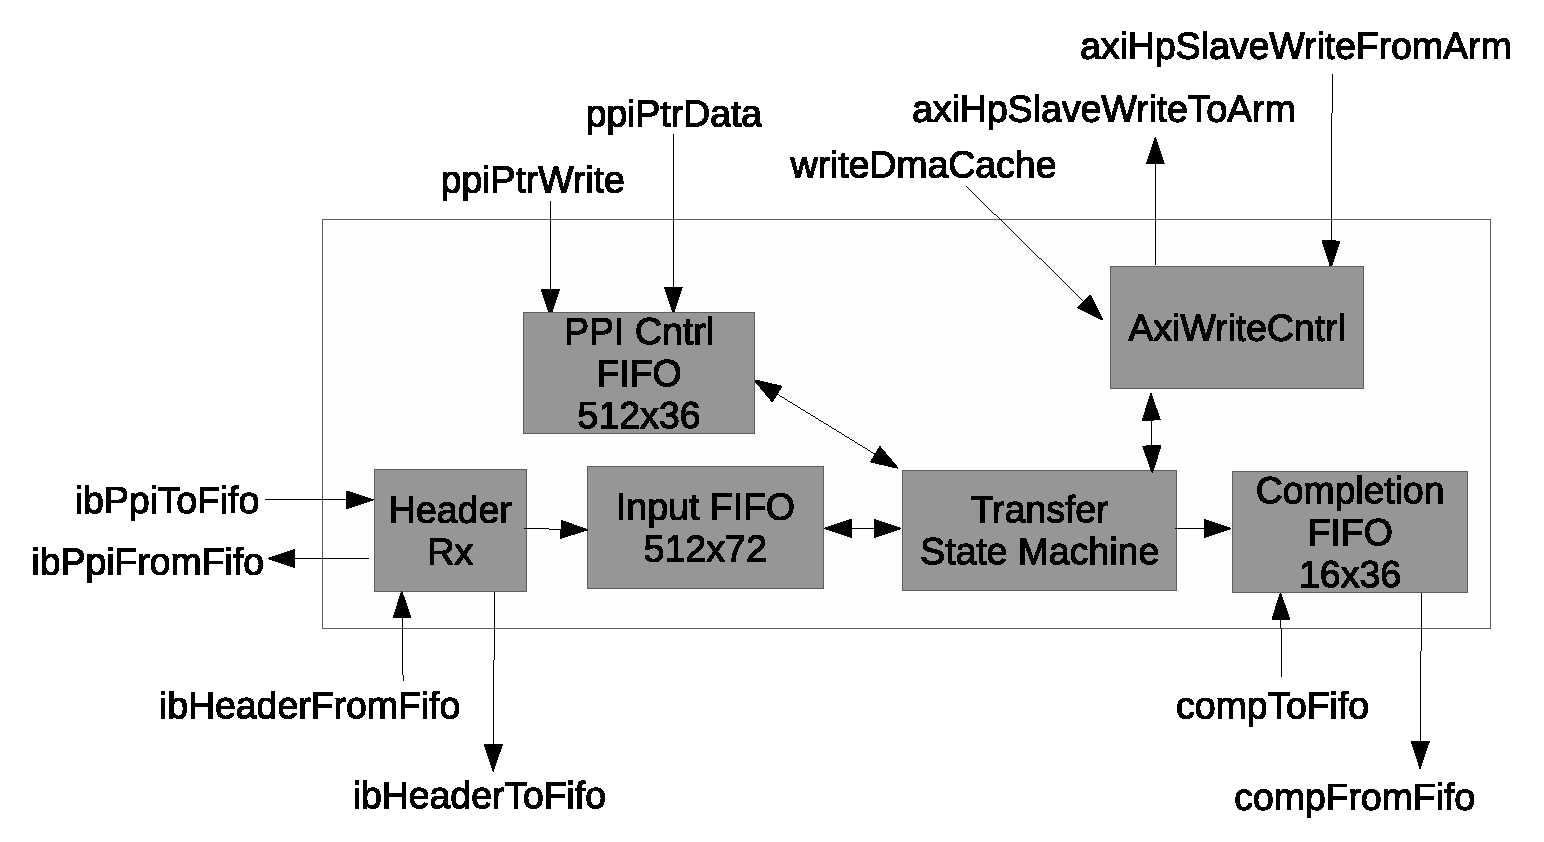
\psfig{file=images/arm_g3_ib_ppi.eps,scale=0.50}
   \caption{Inbound PPI Controller Block Diagram}
   \label{fig:ib_ppi_block}
\end{figure}

\subsubsection{Inbound PPI Receive Control}

When software wishes to initiate the reception of an inbound PPI payload it will write a receive control
descriptor to the inbound PPI control FIFO. The receive control descriptor requires three separate 
writes to the associated FIFO. Bits 35:32 of the FIFO entry are generated by adjusting offset address 
within the FIFO address space.

The format of the inbound PPI receive control descriptor is shown in table \ref{tab:ib_ppi_cntrl}.

\begin{table}[H]
\small
\centering
   \begin{tabular}{| l | l | l | l | l | l | } 
      \hline \textbf{DWord} & \textbf{Bits} & \textbf{Name} & \textbf{Description} \\
      \hline 0              & 35:33         & unused        & ignored                           \\
      \hline 0              & 32            & IbDrop        & Set this bit to discard frame     \\
      \hline 0              & 31:0          & IbAddr        & Inbound frame destination address \\
      \hline 1              & 35:33         & unused        & ignored                           \\
      \hline 1              & 32            & CompEn        & Set this bit to enable completion record generation \\
      \hline 1              & 31:0          & MaxLength     & Maximum length for inbound frame  \\
      \hline 2              & 35:32         & CompIndex     & Completion FIFO selection index.  \\
                            &               &               & Valid values are 0 - 11.          \\
      \hline 2              & 31:0          & CompId        & Id value for completion record    \\
      \hline
   \end{tabular}
   \caption{Inbound PPI Receive Descriptor}
   \label{tab:ib_ppi_cntrl}
\end{table}

\subsubsection{Inbound PPI Receive Completion Record}

When the inbound frame DMA operation is completed, the inbound PPI engine has the ability to add a completion record to one of the 11 
completion FIFOs. The CompEn bit in the inbound receive control descriptor determines if a completion record is 
generated and the CompIndex field determines which of the 11 FIFOs to route the completion record to. The value written 
to the completion record is defined in the CompId field of the inbound receive control record. When the IbDrop bit is set
a completion record is not generated.

The format of the receive completion record is shown in table \ref{tab:ib_ppi_comp}.

\begin{table}[H]
\small
\centering
   \begin{tabular}{| l | l | l | l | l | } 
      \hline \textbf{Bits} & \textbf{Name} & \textbf{Description} \\
      \hline 31:0          & CompId        & Completion ID field from receive descriptor.                           \\
      \hline
   \end{tabular}
   \caption{Inbound PPI Receive Completion Descriptor}
   \label{tab:ib_ppi_comp}
\end{table}

\subsubsection{Inbound PPI Flow Control}

The inbound PPI module will assert the pause signal to the PPI client firmware when the inbound frame FIFO has less than 255 entries (out of 512)
available. The pause signal will also be asserted when the associated inbound header FIFO also has less than 255 entires (out of 512) available.

\subsection{AXI Write Controller (ArmRceG3AxiWriteCntrl.vhd)}
\label{subsec:ArmRceG3AxiWriteCntrl}

The AXI write control module serves two purposes. The first is to provide arbitration between AXI masters in cases
where more than one write source is attached to a shared AXI bus. The second is to provide address and data FIFOs 
between the attached write state machine and the processor's AXI interface. This simplifies the implementation of the 
attached state machine and decouples the AXI interface flow control handshaking from the bursting nature of the 
attached write state machines.

The AXI write controller supports two modes of operation. The first supports 9 separate write masters when
used in the inbound controller block (see section \ref{subsec:ArmRceG3IbCntrl}). The second supports a single 
master when used in the in the inbound PPI controller (see section \ref{subsec:ArmRceG3IbPpi}).
When only master is attached the arbitration stage is optimized away to reduce latency.

\subsubsection{AXI Write Controller Interfaces}

The generic ports for the AXI write controller module are shown in table \ref{tab:axi_write_generics}.

\begin{table}[H]
\small
\centering
   \begin{tabular}{| l | l | l | l | }
      \hline \textbf{Value} & \textbf{Type} & \textbf{Default} & \textbf{Description} \\
      \hline TPD\_G          & time     & 1 ns & Synchronous signal delay value for simulation.    \\
      \hline CHAN\_CNT\_G    & positive & 1    & Number of write master channels. 1 or 9.        \\
      \hline
   \end{tabular}
   \caption{ArmRceG3AxiWriteCntrl Generics}
   \label{tab:axi_write_generics}
\end{table}

The signal ports for the AXI write controller module are shown in table \ref{tab:axi_write_signals}.
Any records referenced in this table are described in detail in section \ref{sec:vhdl_records}. 

\begin{table}[H]
\small
\centering
   \begin{tabular}{| l | l | l | l | l | } 
      \hline \textbf{Signal}            & \textbf{Type} & \textbf{Width} & \textbf{Direction} & \textbf{Description} \\
      \hline axiClk                     & Logic                                                          & 1            & In  & AXI interface clock       \\
      \hline axiClkRst                  & Logic                                                          & 1            & In  & AXI interface reset       \\
      \hline axiSlaveWriteFromArm       & \hyperref[subsec:AxiWriteSlaveType]{AxiWriteSlaveType}         & 1            & In  & AXI bus write from ARM     \\
      \hline axiSlaveWriteToArm         & \hyperref[subsec:AxiWriteMasterType]{AxiWriteMasterType}       & 1            & Out & AXI bus write to ARM       \\
      \hline writeDmaCache              & Logic                                                          & 4            & In  & Write DMA cache configuration \\
      \hline axiWriteToCntrl            & \hyperref[subsec:AxiWriteToCntrlType]{AxiWriteToCntrlType}     & CHAN\_CNT\_G & In  & Write structure to master  \\
      \hline axiWriteFromCntrl          & \hyperref[subsec:AxiWriteFromCntrlType]{AxiWriteFromCntrlType} & CHAN\_CNT\_G & Out & Write structure from master \\
      \hline
   \end{tabular}
   \caption{ArmRceG3AxiWriteCntrl Signals}
   \label{tab:axi_write_signals}
\end{table}

\subsubsection{Axi Write Controller Block Diagram}

The AXI write controller contains an arbitration block which selects between one of 9 possible AXI masters. Address data and write data
are buffered in separate 36-bit x 512 entry FIFOs. Address and data engines convert the address and data FIFO entries into transactions on the AXI bus.

\begin{figure}[H]
   \centering
   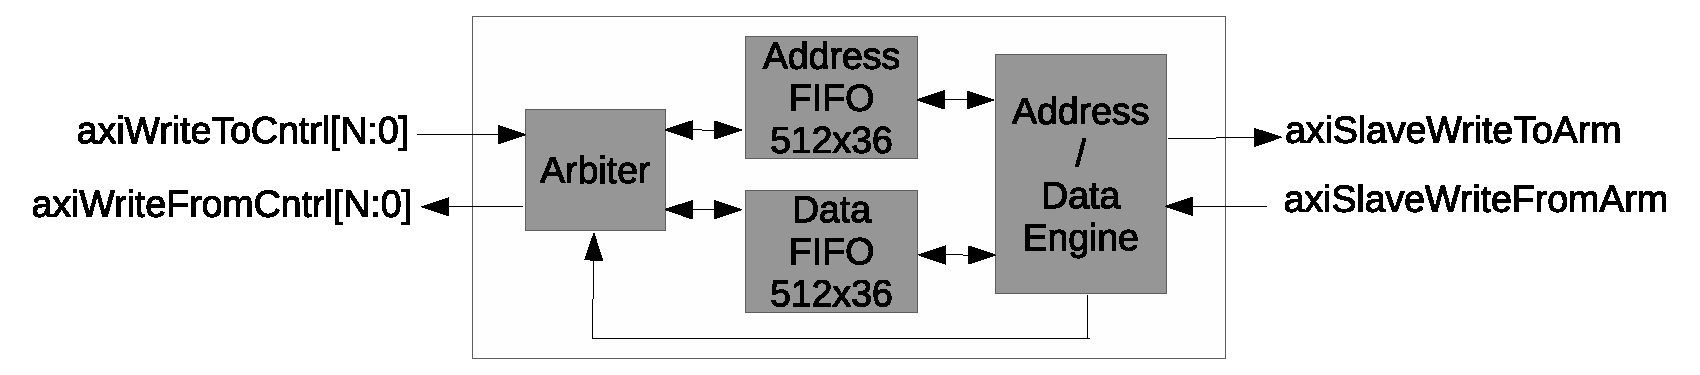
\psfig{file=images/arm_g3_axi_write.eps,scale=0.50}
   \caption{Axi Write Controller Block Diagram}
   \label{fig:axi_write_block}
\end{figure}

\subsection{Outbound Controller (ArmRceG3ObCntrl.vhd)}
\label{subsec:ArmRceG3ObCntrl}

The outbound controller module is a wrapper that contains four instances of the outbound header FIFO block and a single
instances of the AXI read control block. 

\subsubsection{Outbound Controller Interfaces}

The generic ports for the outbound controller module are shown in table \ref{tab:ob_cntrl_generics}.

\begin{table}[H]
\small
\centering
   \begin{tabular}{| l | l | l | l | }
      \hline \textbf{Value} & \textbf{Type} & \textbf{Default} & \textbf{Description} \\
      \hline TPD\_G          & time     & 1 ns & Synchronous signal delay value for simulation.    \\
      \hline
   \end{tabular}
   \caption{ArmRceG3ObCntrl Generics}
   \label{tab:ob_cntrl_generics}
\end{table}

The signal ports for the outbound controller module are shown in table \ref{tab:ob_cntrl_signals}.
Any records referenced in this table are described in detail in section \ref{sec:vhdl_records}. 

\begin{table}[H]
\small
\centering
   \begin{tabular}{| l | l | l | l | l | } 
      \hline \textbf{Signal}            & \textbf{Type} & \textbf{Width} & \textbf{Direction} & \textbf{Description} \\
      \hline axiClk                     & Logic                                                        & 1  & In  & AXI interface clock       \\
      \hline axiClkRst                  & Logic                                                        & 1  & In  & AXI interface reset       \\
      \hline axiAcpSlaveReadFromArm     & \hyperref[subsec:AxiReadSlaveType]{AxiReadSlaveType}         & 1  & In  & AXI ACP bus write from ARM     \\
      \hline axiAcpSlaveReadToArm       & \hyperref[subsec:AxiReadMasterType]{AxiReadMasterType}       & 1  & Out & AXI ACP bus write to ARM       \\
      \hline headerPtrWrite             & Logic                                                        & 4  & In  & Header pointer write enable \\
      \hline headerPtrData              & Logic                                                        & 36 & In  & Header pointer write data \\
      \hline freePtrSel                 & Logic                                                        & 3  & In  & Free list read select. \\
      \hline freePtrData                & Logic                                                        & 32 & Out & Free list read data. \\
      \hline freePtrRd                  & Logic                                                        & 1  & In  & Free list read enable. \\
      \hline freePtrRdValid             & Logic                                                        & 1  & Out & Free list read data valid. \\
      \hline memBaseAddress             & Logic                                                        & 14 & In  & Memory base address \\
      \hline fifoEnable                 & Logic                                                        & 4  & In  & FIFO enable control \\
      \hline readDmaCache               & Logic                                                        & 4  & In  & Read DMA cache configuration \\
      \hline obHeaderToFifo             & \hyperref[subsec:ObHeaderToFifoType]{ObHeaderToFifoType}     & 4  & In  & Outbound header FIFO inputs    \\
      \hline obHeaderFromFifo           & \hyperref[subsec:ObHeaderFromFifoType]{ObHeaderFromFifoType} & 4  & Out & Outbound header FIFO outputs   \\
      \hline
   \end{tabular}
   \caption{ArmRceG3ObCntrl Signals}
   \label{tab:ob_cntrl_signals}
\end{table}

\subsubsection{Outbound Controller Block Diagram}

The block diagram of the outbound controller module is shown in figure \ref{fig:ob_cntrl_block}. The following sub modules
exist within the module and are described in greater detail later in this document:

\begin{itemize}
   \item ArmRceG3ObHeaderFifo: Inbound header transfer FIFO and control logic (section \ref{subsec:ArmRceG3IbHeaderFifo})
   \item ArmRceG3AxiReadCntrl: AXI write controller (section \ref{subsec:ArmRceG3AxiWriteCntrl})
\end{itemize}

The outbound controller module also contains 4 outbound free list FIFOs.

\begin{figure}[H]
   \centering
   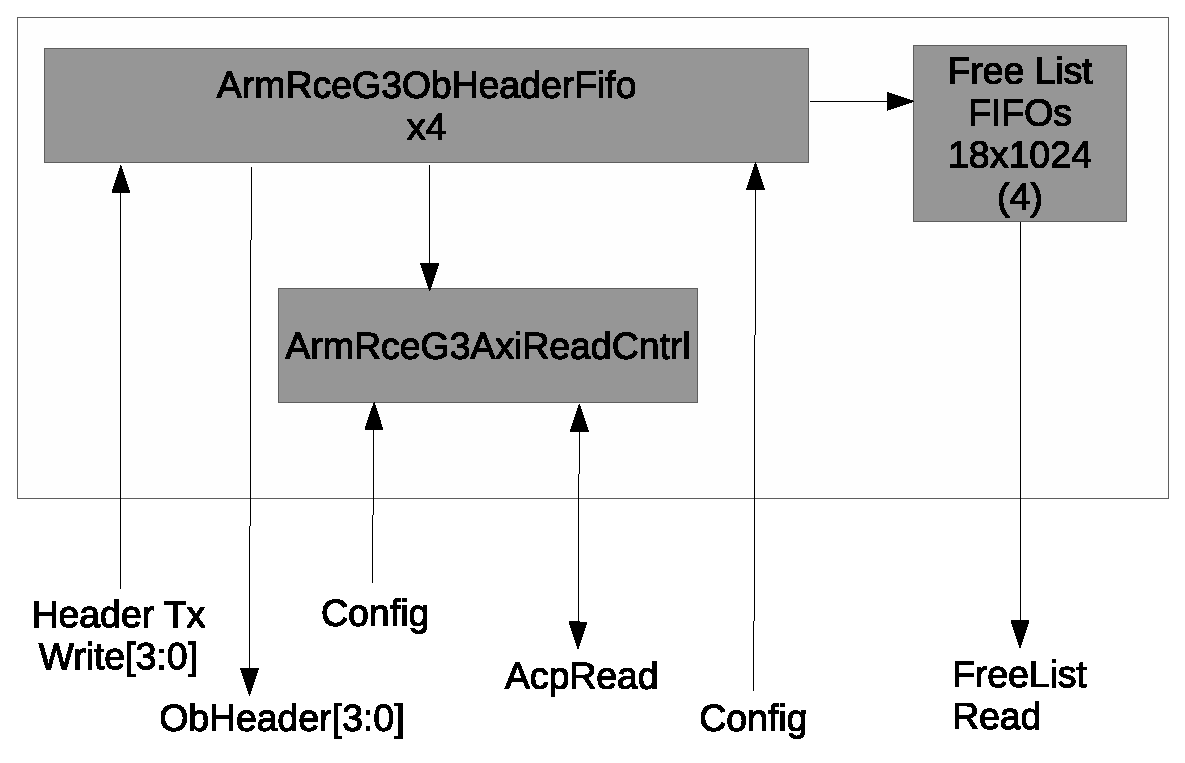
\psfig{file=images/arm_g3_ob_cntrl.eps,scale=0.50}
   \caption{Outbound Controller Block Diagram}
   \label{fig:ob_cntrl_block}
\end{figure}

\subsection{Outbound Header FIFO (ArmRceG3ObHeaderFifo.vhd)}
\label{subsec:ArmRceG3ObHeaderFifo}

The function of the outbound header FIFO module is to transfer PPI header data from OCM to the outbound PPI
module (see section \ref{subsec:ArmRceG3ObPpi}).

The transfer is started when software writes a transmit descriptor to the transmit list FIFO. The transfer state
machine will then exit the idle state, pull the offset address and length from the transmit descriptor and begin reading
from the OCM. Each read request is a fixed size of 32-bytes of data regardless of the length. The outbound 
transfer state machine will queue as many read requests as it has space left in it's outbound FIFO. Anytime the
transfer engine pauses for flow control it will release control of the AXI bus allowing it to be re-arbitrated. 

When the transmission operation is complete the offset address from the transmit descriptor will be placed back
on the free list.

The outbound header FIFO will not operate if the associated fifoEnable configuration bit is not set.

\subsubsection{Outbound Header FIFO Interfaces}

The generic ports for the outbound header FIFO module are shown in table \ref{tab:ob_header_generics}.

\begin{table}[H]
\small
\centering
   \begin{tabular}{| l | l | l | l | }
      \hline \textbf{Value} & \textbf{Type} & \textbf{Default} & \textbf{Description} \\
      \hline TPD\_G          & time     & 1 ns & Synchronous signal delay value for simulation.    \\
      \hline
   \end{tabular}
   \caption{ArmRceG3ObHeaderFifo Generics}
   \label{tab:ob_header_generics}
\end{table}

The signal ports for the outbound header FIFO module are shown in table \ref{tab:ob_header_signals}.
Any records referenced in this table are described in detail in section \ref{sec:vhdl_records}. 

\begin{table}[H]
\small
\centering
   \begin{tabular}{| l | l | l | l | l | } 
      \hline \textbf{Signal}    & \textbf{Type} & \textbf{Width} & \textbf{Direction} & \textbf{Description} \\
      \hline axiClk             & Logic                                                        & 1  & In  & AXI interface clock       \\
      \hline axiClkRst          & Logic                                                        & 1  & In  & AXI interface reset       \\
      \hline axiReadToCntrl     & \hyperref[subsec:AxiReadToCntrlType]{AxiReadToCntrlType}     & 1  & Out & Read structure to controller \\
      \hline axiReadFromCntrl   & \hyperref[subsec:AxiReadFromCntrlType]{AxiReadFromCntrlType} & 1  & In  & Read structure from controller \\
      \hline headerPtrWrite     & Logic                                                        & 1  & In  & Header pointer write enable \\
      \hline headerPtrData      & Logic                                                        & 36 & In  & Header pointer write data \\
      \hline freePtrWrite       & Logic                                                        & 1  & Out & Header free list write  \\
      \hline freePtrData        & Logic                                                        & 32 & Out & Header free list data   \\
      \hline memBaseAddress     & Logic                                                        & 14 & In  & Memory base address \\
      \hline fifoEnable         & Logic                                                        & 1  & In  & FIFO enable control \\
      \hline headerReadDmaId    & Logic                                                        & 3  & In  & Header read DMA ID \\
      \hline obHeaderToFifo     & \hyperref[subsec:ObHeaderToFifoType]{ObHeaderToFifoType}     & 1  & In  & Outbound header FIFO inputs    \\
      \hline obHeaderFromFifo   & \hyperref[subsec:ObHeaderFromFifoType]{ObHeaderFromFifoType} & 1  & Out & Outbound header FIFO outputs   \\
      \hline
   \end{tabular}
   \caption{ArmRceG3ObHeaderFifo Signals}
   \label{tab:ob_header_signals}
\end{table}

\subsubsection{Outbound Header FIFO Block Diagram}

The outbound header FIFO module consists of a 72-bit wide by 512 entry deep input FIFO and a transfer state machine. A 36-bit x 512 entry FIFO is used
for outbound transmit control.

\begin{figure}[H]
   \centering
   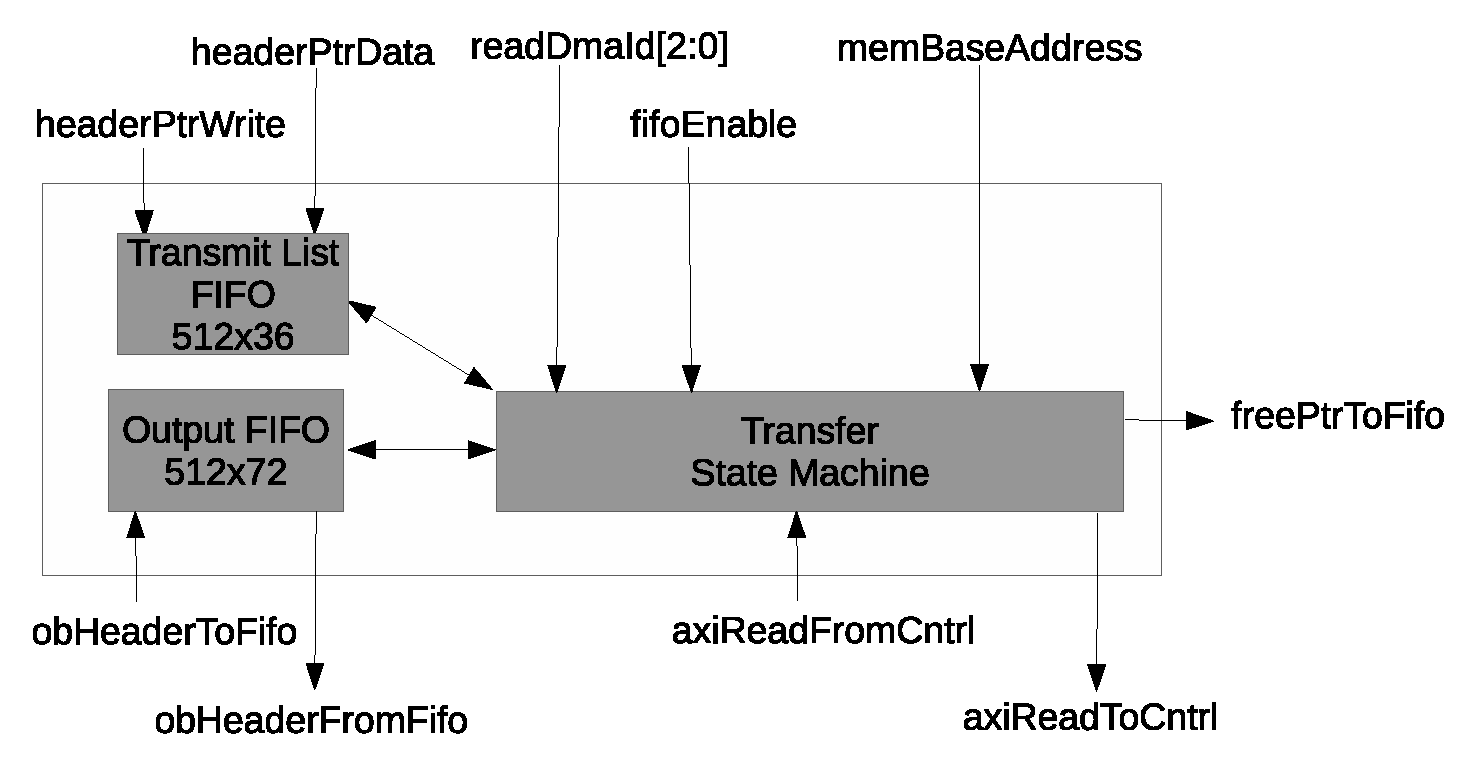
\psfig{file=images/arm_g3_ob_head_block.eps,scale=0.50}
   \caption{Outbound Header FIFO Block Diagram}
   \label{fig:ob_head_block}
\end{figure}

\subsubsection{Outbound Header Free List}

Each of the outbound header FIFOs provide a descriptor free list.  This free list is implemented in a local FIFO which is read over the local bus. 
At startup the software will populate the free list by submitting transmit descriptors with the transfer bit set (described in section \ref{subsec:ob_tx_desc}). 
During normal operation the software will pull a free transmit buffer from the free list and provide it to the header engine as part of the transmit descriptor. 
When the transmit operation has completed the address will be returned to the free list. 

The format of the outbound free list entry is shown in table \ref{tab:ob_tx_flist}.

\begin{table}[H]
\small
\centering
   \begin{tabular}{| l | l | l | l | l | } 
      \hline \textbf{Bits} & \textbf{Name} & \textbf{Description} \\
      \hline 31            & valid         & Bit to indicate if read entry is valid. \\
      \hline 30:18         & unused        & Read as zero.                                                        \\
      \hline 17:3          & address       & This field contains the offset address for the outbound header    \\
                           &               & free list. This address is relative to the configured base address \\
                           &               & and must be cache line aligned.                                    \\
      \hline 2:0           & address       & These bits are always zero.                                                \\
      \hline
   \end{tabular}
   \caption{Outbound Header Free List Entry}
   \label{tab:ob_tx_flist}
\end{table}

\subsubsection{Outbound Header Transmit Descriptor}
\label{subsec:ob_tx_desc}

An outbound header transmission is started by writing a descriptor to the appropriate header transmit FIFO. 
Since the upper data bits (35:32) of the transmit FIFOs are not used only the base address per each FIFO is utilized. 
Each transmit FIFO is capable of holding 511 free list entries. 
The format of the transmit header descriptor is shown in table \ref{tab:ob_tx_desc}.

\begin{table}[H]
\small
\centering
   \begin{tabular}{| l | l | l | l | l | } 
      \hline \textbf{Bits} & \textbf{Name} & \textbf{Description} \\
      \hline 31            & unused        & unused bit                                                           \\
      \hline 30            & transfer      & When this bit is set the passed address will be passed directly      \\
                           &               & to the free list without data transmission.                          \\
      \hline 29            & mgmt          & mgmt field for outbound frame                                        \\ 
      \hline 28:26         & htype         & frame type field for outbound frame                                  \\
      \hline 25:18         & length        & Length of header portion of outbound frame. One based length (1=1, 2=2) \\
                           &               & Specified in number of 64-bit quad words to transfer.                \\
      \hline 17:3          & address       & This field contains the offset address for the outbound header       \\
                           &               & transmission. This address is relative to the configured base address  \\
                           &               & and must be cache line aligned.                                        \\
      \hline 2:0           & address       & These bits are always zero.                                            \\
      \hline
   \end{tabular}
   \caption{Outbound Header Transmit Descriptor}
   \label{tab:ob_tx_desc}
\end{table}

When the outbound header transmission has completed the address will be returned to the outbound header free list Quad Word FIFO.

\subsection{Outbound PPI Controller (ArmRceG3ObPpi.vhd)}
\label{subsec:ArmRceG3ObPpi}

The outbound PPI controller transmits a complete PPI frame by first forwarding the contents of the outbound header FIFO and attaching an optional
payload. The last 4 32-bit words contained in the header received from the outbound header FIFO are used as a PPI transmit descriptor and are
not included as part of the outbound frame. The contents of this descriptor are described in table \ref{tab:ob_ppi_cntrl}.
When the outbound DMA operation has completed, a completion descriptor is written to a targeted completion FIFO. The contents of this completion 
descriptor are detailed in table \ref{tab:ob_ppi_comp}.

Each outbound PPI engine is attached to one of the four HP AXI read interfaces. This dedicated connection means that the outbound PPI engine
can assume complete ownership of the interface. A simplified version of the AXI read controller (described in section \ref{subsec:ArmRceG3AxiReadCntrl})
is instantiated in the module in order to simplify the state machine and improve timing performance. In order to ensure AXI bus efficiency all read 
transfers are a fixed size of 128 bytes.

A byte realignment block is used to allow byte aligned transfer sizes and start addresses. The transfer size of the initial read block at the start 
of a new payload frame is adjusted in order to align the remaining transfers to 128 byte memory boundaries. This is done to ensure that none of the read 
transfers cross a 4-KByte boundary.

\subsubsection{Outbound PPI Controller Interfaces}

The generic ports for the outbound PPI module are shown in table \ref{tab:ob_ppi_generics}.

\begin{table}[H]
\small
\centering
   \begin{tabular}{| l | l | l | l | }
      \hline \textbf{Value} & \textbf{Type} & \textbf{Default} & \textbf{Description} \\
      \hline TPD\_G          & time     & 1 ns & Synchronous signal delay value for simulation.    \\
      \hline
   \end{tabular}
   \caption{ArmRceG3ObPpi Generics}
   \label{tab:ob_ppi_generics}
\end{table}

The signal ports for the outbound PPI module are shown in table \ref{tab:ob_ppi_signals}.
Any records referenced in this table are described in detail in section \ref{sec:vhdl_records}. 

\begin{table}[H]
\small
\centering
   \begin{tabular}{| l | l | l | l | l | } 
      \hline \textbf{Signal}            & \textbf{Type} & \textbf{Width} & \textbf{Direction} & \textbf{Description} \\
      \hline axiClk                     & Logic                                                            & 1  & In       & AXI interface clock       \\
      \hline axiClkRst                  & Logic                                                            & 1  & In       & AXI interface reset       \\
      \hline axiHpSlaveReadFromArm      & \hyperref[subsec:AxiReadSlaveType]{AxiReadSlaveType}             & 1  & In       & AXI HP bus write from ARM \\
      \hline axiHpSlaveReadToArm        & \hyperref[subsec:AxiReadMasterType]{AxiReadMasterType}           & 1  & Out      & AXI HP bus write to ARM  \\
      \hline obHeaderToFifo             & \hyperref[subsec:ObHeaderToFifoType]{ObHeaderToFifoType}         & 1  & Out      & Outbound header FIFO outputs   \\
      \hline obHeaderFromFifo           & \hyperref[subsec:ObHeaderFromFifoType]{ObHeaderFromFifoType}     & 1  & In       & Outbound header FIFO inputs   \\
      \hline readDmaCache               & Logic                                                            & 4  & In       & Read DMA cache configuration \\
      \hline compFromFifo               & \hyperref[subsec:CompFromFifoType]{CompFromFifoType}             & 1  & Out      & Completion FIFO outputs   \\
      \hline compToFifo                 & \hyperref[subsec:CompToFifoType]{CompToFifoType}                 & 1  & In       & Completion FIFO inputs   \\
      \hline obPpiClk                   & Logic                                                            & 1  & In       & Outbound PPI clocks  \\
      \hline obPpiToFifo                & \hyperref[subsec:ObPpiToFifoType]{ObPpiToFifoType}               & 1  & In       & Outbound PPI input signals \\
      \hline obPpiFromFifo              & \hyperref[subsec:ObPpiFromFifoType]{ObPpiFromFifoType}           & 1  & Out      & Outbound PPI outout signals \\
      \hline
   \end{tabular}
   \caption{ArmRceG3ObPpi Signals}
   \label{tab:ob_ppi_signals}
\end{table}

\subsubsection{Outbound PPI Block Diagram}

The outbound PPI controller module consists of a transfer state machine which is bridged to the AXI bus using an ArmRceG3AxiReadCntrl (see section \ref{subsec:ArmRceG3AxiWriteCntrl})
module. Transmit control descriptors are buffered using a 36-bit x 512 entry transmit control FIFO. Outbound data is buffered in a 72-bit x 512 entry FIFO. 
A 36-bit by 16 entry FIFO serves as a staging FIFO for completion records. 

\begin{figure}[H]
   \centering
   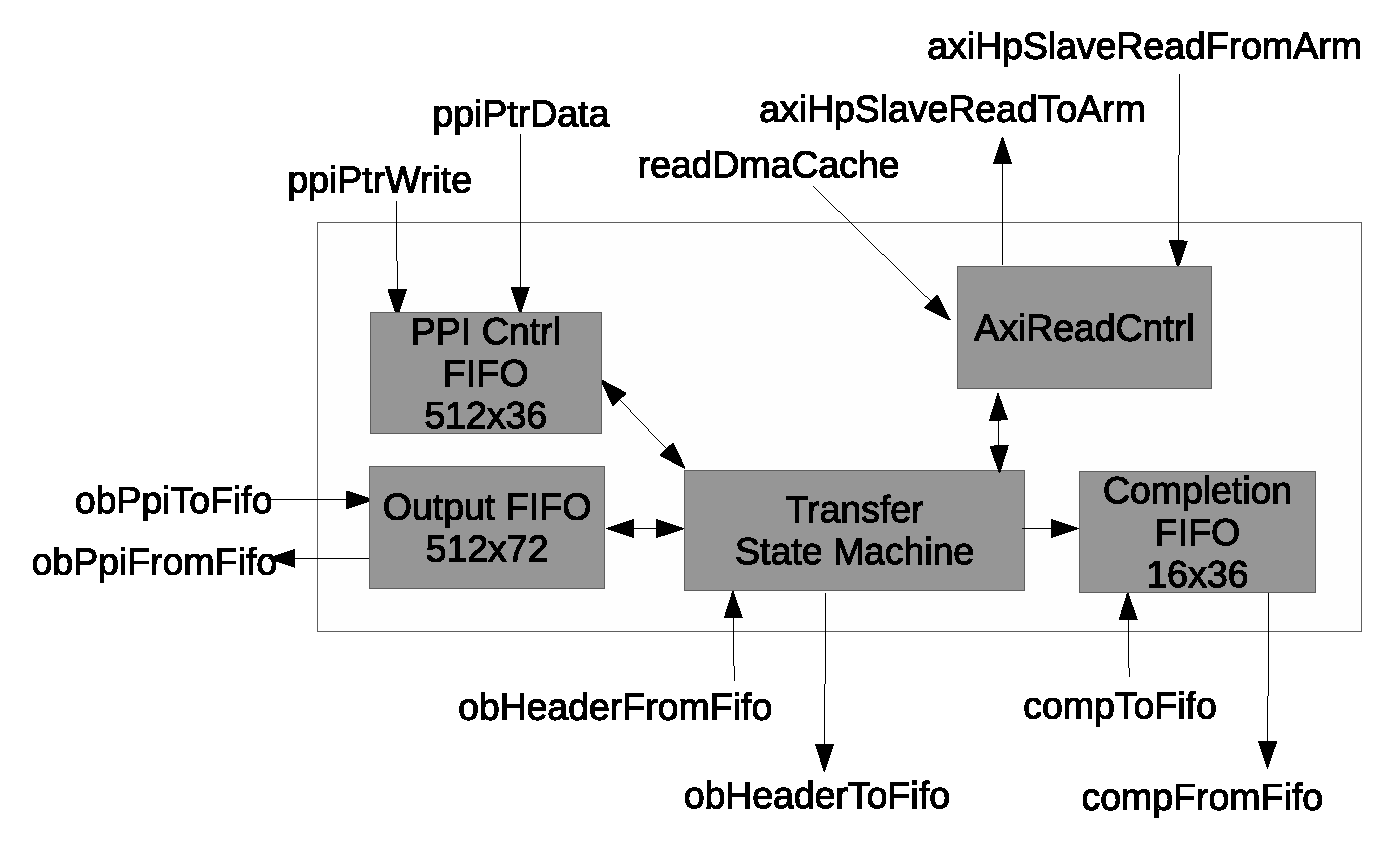
\psfig{file=images/arm_g3_ob_ppi.eps,scale=0.50}
   \caption{Outbound PPI Block Diagram}
   \label{fig:ob_ppi_block}
\end{figure}

\subsubsection{Outbound PPI Transmit Control}

Outbound PPI frame transmission is controlled by the last four 32-bit dual words in the outbound PPI header frame. 
These four words are form the outbound PPI transmit descriptor and are not included in the outbound frame. 

The format of the outbound PPI transmit control descriptor is shown in table \ref{tab:ob_ppi_cntrl}.

\begin{table}[H]
\small
\centering
   \begin{tabular}{| l | l | l | l | l | l | } 
      \hline \textbf{DWord} & \textbf{Bits} & \textbf{Name} & \textbf{Description} \\
      \hline 0              & 31:0          & ObAddr        & Outbound frame source address     \\
      \hline 1              & 31:0          & ObLength      & Length of outbound frame in bytes \\
      \hline 2              & 31:0          & CompId        & Id value for completion record    \\
      \hline 3              & 31:6          & unused        & ignored                           \\
      \hline 3              & 5             & ObEmpty       & Set this bit to indicate that frame payload is empty. \\
      \hline 3              & 4             & CompEn        & Set this bit to enable completion record generation \\
      \hline 3              & 3:0           & CompIndex     & Completion FIFO selection index.  \\
                            &               &               & Valid values are 0 - 11.          \\
      \hline
   \end{tabular}
   \caption{Outbound PPI Transmit Descriptor}
   \label{tab:ob_ppi_cntrl}
\end{table}

\subsubsection{Outbound PPI Transmit Completion Record}

When the outbound frame DMA operation is completed, the outbound PPI engine has the ability to add a completion record to one of the 11 
completion FIFOs. The CompEn bit in the outbound transmit control descriptor determines if a completion record is 
generated and the CompIndex field determines which of the 11 FIFOs to route the completion record to. The value written 
to the completion record is defined in the CompId field of the outbound transmit control record. 

The format of the receive completion record is shown in table \ref{tab:ob_ppi_comp}.

\begin{table}[H]
\small
\centering
   \begin{tabular}{| l | l | l | l | l | } 
      \hline \textbf{Bits} & \textbf{Name} & \textbf{Description} \\
      \hline 31:0          & CompId        & Completion ID field from transmit descriptor.                           \\
      \hline
   \end{tabular}
   \caption{Outbound PPI Transmit Completion Descriptor}
   \label{tab:ob_ppi_comp}
\end{table}

\subsection{AXI Read Controller (ArmRceG3AxiReadCntrl.vhd)}
\label{subsec:ArmRceG3AxiReadCntrl}

Similar to the AXI write control module, the AXI read controller provides arbitration between AXI masters in cases
where more than one read source is attached to a shared AXI bus. It also provides an address FIFO 
between the attached read state machine and the processor's AXI interface. Returned read data is first
passed to a FIFO to decouple flow control which may be originated by the attached read state machine(s) from
the signals on the AXI bus interface.

The AXI read controller supports two modes of operation. The first supports 4 separate write masters when
used in the outbound controller block (see section \ref{subsec:ArmRceG3IbCntrl}). The second supports a single 
master when used in the in the outbound PPI controller (see section \ref{subsec:ArmRceG3ObPpi}).
When only master is attached the arbitration stage is optimized away to reduce latency.

\subsubsection{AXI Read Controller Interfaces}

The generic ports for the AXI read controller module are shown in table \ref{tab:axi_read_generics}.

\begin{table}[H]
\small
\centering
   \begin{tabular}{| l | l | l | l | }
      \hline \textbf{Value} & \textbf{Type} & \textbf{Default} & \textbf{Description} \\
      \hline TPD\_G          & time     & 1 ns & Synchronous signal delay value for simulation.    \\
      \hline CHAN\_CNT\_G    & positive & 1    & Number of read master channels. 1 or 4.        \\
      \hline
   \end{tabular}
   \caption{ArmRceG3AxiReadCntrl Generics}
   \label{tab:axi_read_generics}
\end{table}

The signal ports for the AXI read controller module are shown in table \ref{tab:axi_read_signals}.
Any records referenced in this table are described in detail in section \ref{sec:vhdl_records}. 

\begin{table}[H]
\small
\centering
   \begin{tabular}{| l | l | l | l | l | } 
      \hline \textbf{Signal}            & \textbf{Type} & \textbf{Width} & \textbf{Direction} & \textbf{Description} \\
      \hline axiClk                     & Logic                                                            & 1  & In       & AXI interface clock       \\
      \hline axiClkRst                  & Logic                                                            & 1  & In       & AXI interface reset       \\
      \hline axiSlaveReadFromArm        & \hyperref[subsec:AxiReadSlaveType]{AxiReadSlaveType}             & 1  & In       & AXI bus read from ARM     \\
      \hline axiSlaveReadToArm          & \hyperref[subsec:AxiReadMasterType]{AxiReadMasterType}           & 1  & Out      & AXI bus read to ARM       \\
      \hline readDmaCache               & Logic                                                            & 4  & In       & Read DMA cache configuration \\
      \hline axiReadToCntrl             & \hyperref[subsec:AxiReadToCntrlType]{AxiReadToCntrlType}         & CHAN\_CNT\_G & In       & Read structure to master  \\
      \hline axiReadFromCntrl           & \hyperref[subsec:AxiReadFromCntrlType]{AxiReadFromCntrlType}     & CHAN\_CNT\_G & Out      & Read structure from master \\
      \hline
   \end{tabular}
   \caption{ArmRceG3AxiReadCntrl Signals}
   \label{tab:axi_read_signals}
\end{table}

\subsubsection{Axi Read Controller Block Diagram}

The AXI read controller contains an arbitration block which selects between one of 4 possible AXI masters. Address data is 
buffered in a 36-bit x 512 entry FIFO. An address engines converts the address into transactions on the AXI bus. 

\begin{figure}[H]
   \centering
   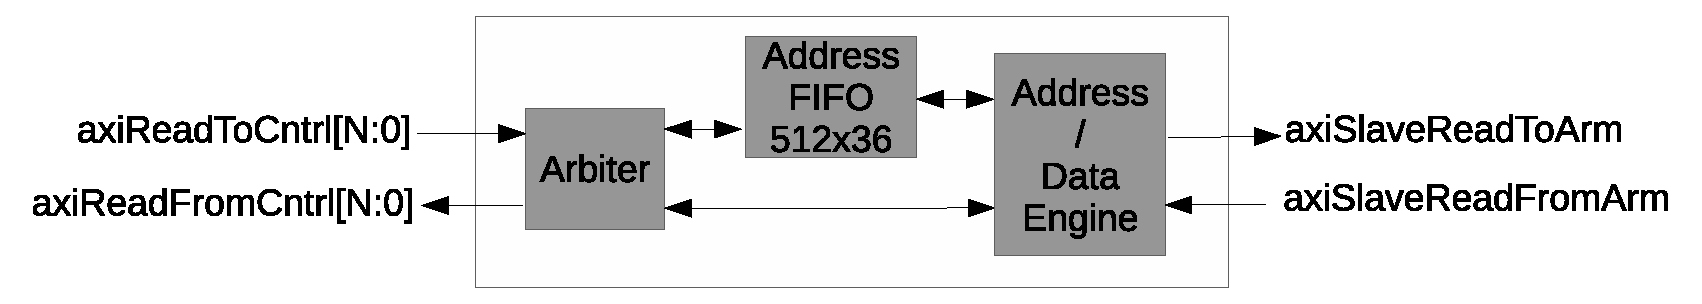
\psfig{file=images/arm_g3_axi_read.eps,scale=0.50}
   \caption{Axi Read Controller Block Diagram}
   \label{fig:axi_read_block}
\end{figure}

\subsection{DMA Completion FIFO Controller (ArmRceG3DmaComp.vhd)}
\label{subsec:ArmRceG3DmaComp}

The purpose of the DMA completion FIFO controller is to accept completion records from the four inbound PPI engines and the four outbound PPI engines. 
Each of the PPI engines has the ability to direct it's completion entries to one of 11 completion FIFOs. Each completion entry is treated independently 
and can be targeted to a different completion FIFO than other completion entries from the same source. 

When a completion FIFOs is non-empty it asserts a ready status bit which can be read over the AXI bus and be configured to trigger an interrupt. 
The mapping of the 11 completion FIFOs to interrupts is described earlier in this document in table \ref{tab:dma_int_mappings}. The contents of
the completion FIFOs are read over the AXI bus. When software reads from the address associated with a completion FIFO the entry at the head of
the queue is returned to software and the contents of the FIFO are advanced. 

The completion engine works by iterating through each of the 8 possible sources, one per clock cycle. When a particular source is selected the
completion record is examined and the destination ID is determined. If the requested destination FIFO is not full the completion entry will 
then be moved to the selected completion FIFO. 

\subsubsection{DMA Completion Mover Interfaces}

The generic ports for the DMA completion mover are shown in table \ref{tab:dma_comp_generics}.

\begin{table}[H]
\small
\centering
   \begin{tabular}{| l | l | l | l | }
      \hline \textbf{Value} & \textbf{Type} & \textbf{Default} & \textbf{Description} \\
      \hline TPD\_G          & time     & 1 ns & Synchronous signal delay value for simulation.    \\
      \hline
   \end{tabular}
   \caption{ArmRceG3DmaComp Generics}
   \label{tab:dma_comp_generics}
\end{table}

The signal ports for the DMA completion mover are shown in table \ref{tab:dma_comp_signals}.
Any records referenced in this table are described in detail in section \ref{sec:vhdl_records}. 

\begin{table}[H]
\small
\centering
   \begin{tabular}{| l | l | l | l | l | } 
      \hline \textbf{Signal}            & \textbf{Type} & \textbf{Width} & \textbf{Direction} & \textbf{Description} \\
      \hline axiClk                     & Logic                                                            & 1  & In       & AXI interface clock       \\
      \hline axiClkRst                  & Logic                                                            & 1  & In       & AXI interface reset       \\
      \hline compFromFifo               & \hyperref[subsec:CompFromFifoType]{CompFromFifoType}             & 8 & In        & Completion FIFO inputs   \\
      \hline compToFifo                 & \hyperref[subsec:CompToFifoType]{CompToFifoType}                 & 8 & Out       & Completion FIFO outputs   \\
      \hline compFifoSel                & Logic                                                            & 4 & In        & FIFO read selection       \\
      \hline compFifoRd                 & Logic                                                            & 1  & In        & FIFO read strobe          \\
      \hline compFifoData               & Logic                                                            & 32 & Out       & FIFO read data            \\
      \hline compFifoValid              & Logic                                                            & 1  & Out       & FIFO read data valid      \\
      \hline compInt                    & Logic                                                            & 11 & Out       & FIFO ready interrupts     \\
      \hline
   \end{tabular}
   \caption{ArmRceG3DmaComp Signals}
   \label{tab:dma_comp_signals}
\end{table}

\subsubsection{DMA Completion Block Diagram}

The DMA completion module consists of a completion engine which transfers data from a series of small inbound header and outbound header 
completion FIFOs to one of 9 independent 36-bit x 512 entry completion FIFOs. A read control block allows the 9 completion to be read from
the local bus.

\begin{figure}[H]
   \centering
   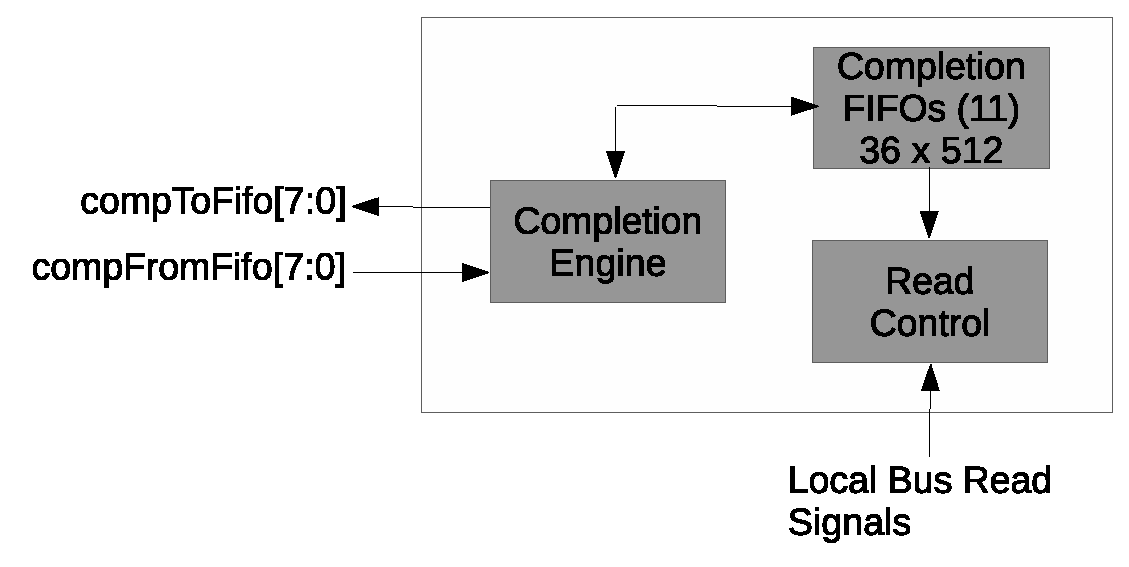
\psfig{file=images/arm_g3_dma_comp.eps,scale=0.50}
   \caption{DMA Completion Block Diagram}
   \label{fig:dma_comp_block}
\end{figure}

\subsection{I2C Controller (ArmRceG3I2c.vhd)}
\label{subsec:ArmRceG3I2c}

The I2C controller block supports the BSI operation by providing a message path between the CPU software and the management I2C bus. Anytime a 
byte is written over the I2C bus the appropriate entry in the I2C BRAM is updated with the data contained in the write. When a complete 32-bit
word is written the FIFO writer block will place the 32-bit value along with the target address in the BSI quad word FIFO. 

A 32-bit value is written over the I2C bus by writing the least significant byte first (offset address 0), followed by the second byte (offset 1)
and third byte (offset 2). When the finally byte (offset 3) is written it's value is combined with the previous three received bytes and added to
the quad word FIFO. Software also has the ability to directly read and write the I2C BRAM. 

The I2C management controller may poll the flow control state of the BSI FIFO by reading from offset address 0x800.

\subsubsection{I2C Controller Interfaces}

The generic ports for the I2C controller are shown in table \ref{tab:i2c_cntrl_generics}.

\begin{table}[H]
\small
\centering
   \begin{tabular}{| l | l | l | l | }
      \hline \textbf{Value} & \textbf{Type} & \textbf{Default} & \textbf{Description} \\
      \hline TPD\_G          & time     & 1 ns & Synchronous signal delay value for simulation.    \\
      \hline
   \end{tabular}
   \caption{ArmRceG3I2c Generics}
   \label{tab:i2c_cntrl_generics}
\end{table}

The signal ports for the I2C controller are shown in table \ref{tab:i2c_cntrl_signals}.
Any records referenced in this table are described in detail in section \ref{sec:vhdl_records}. 

\begin{table}[H]
\small
\centering
   \begin{tabular}{| l | l | l | l | l | } 
      \hline \textbf{Signal}            & \textbf{Type} & \textbf{Width} & \textbf{Direction} & \textbf{Description} \\
      \hline axiClk            & Logic   & 1  & In       & AXI bus clock output               \\
      \hline axiClkRst         & Logic   & 1  & In       & AXI bus clock reset                \\
      \hline localBusMaster    & \hyperref[subsec:LocalBusMasterType]{LocalBusMasterType} & 1      & In        & Local bus input      \\
      \hline localBusSlave     & \hyperref[subsec:LocalBusSlaveType]{LocalBusSlaveType}   & 1      & Out       & Local bus output     \\
      \hline bsiToFifo         & \hyperref[subsec:QWordToFifoType]{QWordToFifoType}       & 1  & Out      & BSI FIFO output signals  \\
      \hline bsiFromFifo       & \hyperref[subsec:QWordFromFifoType]{QWordFromFifoType}   & 1  & In       & BSI FIFO input signals \\
      \hline i2cSda            & Logic         & 1      & inout     & BSI I2C slave data              \\
      \hline i2cScl            & Logic         & 1      & inout     & BSI I2C slave clock             \\
      \hline
   \end{tabular}
   \caption{ArmRceG3I2c Signals}
   \label{tab:i2c_cntrl_signals}
\end{table}

\subsubsection{I2C Controller Block Diagram}

The I2c controller module consists of a I2C slave core which converts I2c bus accesses to local byte transfers. A 2Kbyte dual port block ram 
allows read and write access from either the local bus or the I2C bus. A FIFO write module converts I2C write access to quad word FIFO writes.

\begin{figure}[H]
   \centering
   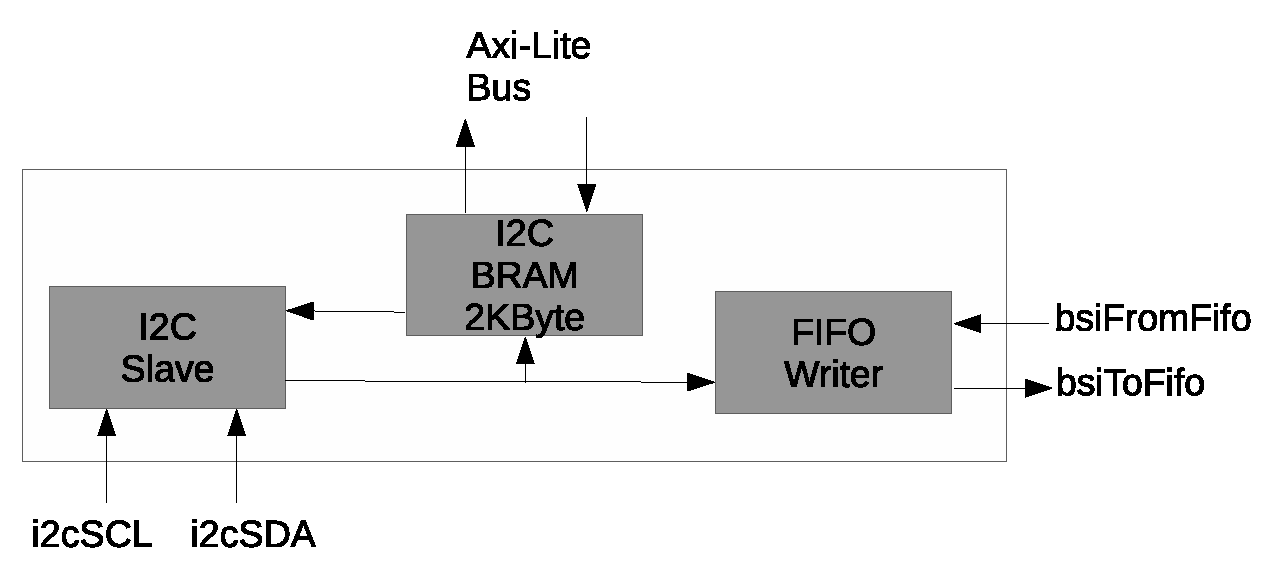
\psfig{file=images/arm_g3_i2c_cntrl.eps,scale=0.50}
   \caption{I2C Controller Block Diagram}
   \label{fig:i2c_cntrl_block}
\end{figure}

\subsubsection{Local Bus Address Space}

RCE software may access the contents of the 2K I2C block ram in the address space 0x8400\_0000 - 0x8400\_07FC.

\subsubsection{I2C Bus Address Space}

The I2C controller may access the contents of the 2K I2C block ram in the address space 0x00 - 0x7FF. 
The BSI Quad Word almost full status appears in bit 0 at address 0x800.
The I2C bus address of the slave device is 0x49.

\subsection{CPU Interface Module (ArmRceG3Cpu.vhd)}
\label{subsec:ArmRceG3Cpu}

The CPU interface module is a wrapper to the processor\_system7\_v4\_02a core provided from Xilinx. 
The interfaces used in the ARM RCE generation 3 core are converted to record types. Unused interfaces are terminated with constants.

Further information and documentation for the processor\_system7 core can be found on the Xilinx website at:
\begin{center}
   \url{http://www.xilinx.com/products/intellectual-property/processing_system7.htm}
\end{center}

\subsubsection{CPU Interfaces}

The generic ports for the CPU core module are shown in table \ref{tab:cpu_core_generics}.

\begin{table}[H]
\small
\centering
   \begin{tabular}{| l | l | l | l | }
      \hline \textbf{Value} & \textbf{Type} & \textbf{Default} & \textbf{Description} \\
      \hline TPD\_G          & time     & 1 ns & Synchronous signal delay value for simulation.    \\
      \hline
   \end{tabular}
   \caption{ArmRceG3Cpu Generics}
   \label{tab:cpu_core_generics}
\end{table}

The signal ports for the I2C controller are shown in table \ref{tab:cpu_core_signals}.
Any records referenced in this table are described in detail in section \ref{sec:vhdl_records}. 

\begin{table}[H]
\small
\centering
   \begin{tabular}{| l | l | l | l | l | } 
      \hline \textbf{Signal}            & \textbf{Type} & \textbf{Width} & \textbf{Direction} & \textbf{Description} \\
      \hline fclkClk3          & Logic   & 1  & Out      & CPU function clock output 3        \\
      \hline fclkClk2          & Logic   & 1  & Out      & CPU function clock output 2        \\
      \hline fclkClk1          & Logic   & 1  & Out      & CPU function clock output 1        \\
      \hline fclkClk0          & Logic   & 1  & Out      & CPU function clock output 0        \\
      \hline fclkRst3          & Logic   & 1  & Out      & CPU function clock reset 3         \\
      \hline fclkRst2          & Logic   & 1  & Out      & CPU function clock reset 2         \\
      \hline fclkRst1          & Logic   & 1  & Out      & CPU function clock reset 1         \\
      \hline fclkRst0          & Logic   & 1  & Out      & CPU function clock reset 0, 100Mhz \\
      \hline axiClk            & Logic   & 1  & In       & Common AXI clock                   \\
      \hline armInt            & Logic   & 16 & In       & Interrupt vector                   \\
      \hline axiGpMasterReset        & Logic                                                      & 2  & Out & GP master port resets           \\
      \hline axiGpMasterWriteFromArm & \hyperref[subsec:AxiWriteMasterType]{AxiWriteMasterType}   & 2  & Out & GP master AXI bus read from ARM \\
      \hline axiGpMasterWriteToArm   & \hyperref[subsec:AxiWriteSlaveType]{AxiWriteSlaveType}     & 2  & In  & GP master AXI bus read to ARM   \\
      \hline axiGpMasterReadFromArm  & \hyperref[subsec:AxiReadMasterType]{AxiReadMasterType}     & 2  & Out & GP master AXI bus read from ARM \\
      \hline axiGpMasterReadToArm    & \hyperref[subsec:AxiReadSlaveType]{AxiReadSlaveType}       & 2  & In  & GP master AXI bus read to ARM   \\
      \hline axiGpSlaveReset         & Logic                                                      & 2  & In  & GP slave port resets            \\
      \hline axiGpSlaveWriteFromArm  & \hyperref[subsec:AxiWriteSlaveType]{AxiWriteSlaveType}     & 2  & Out & GP slave AXI bus read from ARM  \\
      \hline axiGpSlaveWriteToArm    & \hyperref[subsec:AxiWriteMasterType]{AxiWriteMasterType}   & 2  & In  & GP slave AXI bus read to ARM    \\
      \hline axiGpSlaveReadFromArm   & \hyperref[subsec:AxiReadSlaveType]{AxiReadSlaveType}       & 2  & Out & GP slave AXI bus read from ARM  \\
      \hline axiGpSlaveReadToArm     & \hyperref[subsec:AxiReadMasterType]{AxiReadMasterType}     & 2  & In  & GP slave AXI bus read to ARM    \\
      \hline axiAcpSlaveReset        & Logic                                                      & 1  & In  & ACP slave port reset            \\
      \hline axiAcpSlaveWriteFromArm & \hyperref[subsec:AxiWriteSlaveType]{AxiWriteSlaveType}     & 1  & Out & ACP slave AXI bus read from ARM \\
      \hline axiAcpSlaveWriteToArm   & \hyperref[subsec:AxiWriteMasterType]{AxiWriteMasterType}   & 1  & In  & ACP slave AXI bus read to ARM   \\
      \hline axiAcpSlaveReadFromArm  & \hyperref[subsec:AxiReadSlaveType]{AxiReadSlaveType}       & 1  & Out & ACP slave AXI bus read from ARM \\
      \hline axiAcpSlaveReadToArm    & \hyperref[subsec:AxiReadMasterType]{AxiReadMasterType}     & 1  & In  & ACP slave AXI bus read to ARM   \\
      \hline axiHpSlaveReset         & Logic                                                      & 4  & In  & HP slave port resets            \\
      \hline axiAcpSlaveWriteFromArm & \hyperref[subsec:AxiWriteSlaveType]{AxiWriteSlaveType}     & 4  & Out & HP slave AXI bus read from ARM  \\
      \hline axiAcpSlaveWriteToArm   & \hyperref[subsec:AxiWriteMasterType]{AxiWriteMasterType}   & 4  & In  & HP slave AXI bus read to ARM    \\
      \hline axiAcpSlaveReadFromArm  & \hyperref[subsec:AxiReadSlaveType]{AxiReadSlaveType}       & 4  & Out & HP slave AXI bus read from ARM  \\
      \hline axiAcpSlaveReadToArm    & \hyperref[subsec:AxiReadMasterType]{AxiReadMasterType}     & 4  & In  & HP slave AXI bus read to ARM    \\
      \hline ethFromArm              & \hyperref[subsec:EthFromArmType]{EthFromArmType}           & 2  & Out & Ethernet port outputs           \\
      \hline ethToArm                & \hyperref[subsec:EthToArmType]{EthToArmType}               & 2  & In  & Ethernet port inputs            \\
      \hline
   \end{tabular}
   \caption{ArmRceG3Cpu Signals}
   \label{tab:cpu_core_signals}
\end{table}

\newpage
\section{VHDL Record Definitions}
\label{sec:vhdl_records}

This section of the document describes the record types that are used in the ARM RCE Generation 3 Core Module as defined in the VHDL 
source file ArmRceG3Pkg.vhd. All defined record types include an array type (Vector) and an initialization constant (Init). 
An an example the record type AxiReadSlaveType defines a record type, AxiReadSlaveVector can be used to create an array of
AxiReadSlveType types and AxiReadSlaveInit can be used to initialize an AxiReadSlaveType signal or variable.

\subsection{AxiReadMasterType}
\label{subsec:AxiReadMasterType}

The AxiReadMasterType record is used as an output from the Zynq processor read channel master for a specific AXI port. This generic record can be used for the two GP master ports, the two GP slave ports, the ACP slave port and the four HP ports supported by the Xilinx Zynq architecture. 
The AxiReadMasterInit constant can be used to initialize the record and the sub-type AxiReadMasterVector allows an array of this type to be created.

\small 
\begin{verbatim}
   type AxiReadMasterType is record

      -- Read Address channel
      arvalid        : sl;               -- Address valid
      araddr         : slv(31 downto 0); -- Address
      arid           : slv(11 downto 0); -- Channel ID
                                         -- 12 bits for master GP
                                         -- 6  bits for slave GP
                                         -- 3  bits for ACP
                                         -- 6  bits for HP
      arlen          : slv(3  downto 0); -- Transfer count, 0x0=1, 0xF=16
      arsize         : slv(2  downto 0); -- Bytes per transfer, 0x0=1, 0x7=8
      arburst        : slv(1  downto 0); -- Burst Type
                                         -- 0x0 = Fixed address
                                         -- 0x1 = Incrementing address
                                         -- 0x2 = Wrap at cache boundary
      arlock         : slv(1  downto 0); -- Lock control
                                         -- 0x0 = Normal access
                                         -- 0x1 = Exclusive access
                                         -- 0x2 = Locked access
      arprot         : slv(2  downto 0); -- Protection control
                                         -- Bit 0 : 0 = Normal, 1 = Priveleged
                                         -- Bit 1 : 0 = Secure, 1 = Non-secure
                                         -- Bit 2 : 0 = Data access, 1 = Instruction
      arcache        : slv(3  downto 0); -- Cache control
                                         -- Bit 0 : Bufferable
                                         -- Bit 1 : Cachable  
                                         -- Bit 2 : Read allocate enable
                                         -- Bit 3 : Write allocate enable
      arqos          : slv(3  downto 0); -- Xilinx specific, see UG585
      aruser         : slv(4  downto 0); -- ACP only, Xilinx specific, see UG585

      -- Read data channel
      rready         : sl;               -- Master is ready for data

      -- Control 
      rdissuecap1_en : sl;               -- HP only, Xilinx specific, see UG585  

   end record;
\end{verbatim}
\normalsize

\subsection{AxiReadSlaveType}
\label{subsec:AxiReadSlaveType}

The AxiReadSlaveType record is used as an output from the Zynq processor read channel slave for a specific AXI port. This generic record can be used for the two GP master ports, the two GP slave ports, the ACP slave port and the four HP ports supported by the Xilinx Zynq architecture. 
The AxiReadSlaveInit constant can be used to initialize the record and the sub-type AxiReadSlaveVector allows an array of this type to be created.

\small
\begin{verbatim}
   type AxiReadSlaveType is record

      -- Read Address channel
      arready : sl;               -- Slave is ready for address

      -- Read data channel
      rdata   : slv(63 downto 0); -- Read data from slave
                                  -- 32 bits for GP ports
                                  -- 64 bits for other ports
      rlast   : sl;               -- Read data last strobe
      rvalid  : sl;               -- Read data is valid
      rid     : slv(11 downto 0); -- Read data ID
                                  -- 12 for master GP 
                                  -- 6 for slave GP 
                                  -- 3 for ACP 
                                  -- 6 for HP
      rresp   : slv(1  downto 0); -- Read data result
                                  -- 0x0 = Okay
                                  -- 0x1 = Exclusive access okay
                                  -- 0x2 = Slave indicated error 
                                  -- 0x3 = Decode error

      -- Status
      racount : slv(2  downto 0); -- HP only, Xilinx specific, see UG585
      rcount  : slv(7  downto 0); -- HP only, Xilinx specific, see UG585

   end record;
\end{verbatim}
\normalsize

\subsection{AxiWriteMasterType}
\label{subsec:AxiWriteMasterType}

The AxiWriteMasterType record is used as an output from the Zynq processor write channel master for a specific AXI port. This generic record can be used for the two GP master ports, the two GP slave ports, the ACP slave port and the four HP ports supported by the Xilinx Zynq architecture. 
The AxiWriteMasterInit constant can be used to initialize the record and the sub-type AxiWriteMasterVector allows an array of this type to be created.

\small
\begin{verbatim}
   type AxiWriteMasterType is record

      -- Write address channel
      awvalid        : sl;               -- Write address is valid
      awaddr         : slv(31 downto 0); -- Write address
      awid           : slv(11 downto 0); -- Channel ID
                                         -- 12 bits for master GP
                                         -- 6  bits for slave GP
                                         -- 3  bits for ACP
                                         -- 6  bits for HP
      awlen          : slv(3  downto 0); -- Transfer count, 0x0=1, 0xF=16
      awsize         : slv(2  downto 0); -- Bytes per transfer, 0x0=1, 0x7=8
      awburst        : slv(1  downto 0); -- Burst Type
                                         -- 0x0 = Fixed address
                                         -- 0x1 = Incrementing address
                                         -- 0x2 = Wrap at cache boundary
      awlock         : slv(1  downto 0); -- Lock control
                                         -- 0x0 = Normal access
                                         -- 0x1 = Exclusive access
                                         -- 0x2 = Locked access
      arprot         : slv(2  downto 0); -- Protection control
                                         -- Bit 0 : 0 = Normal, 1 = Priveleged
                                         -- Bit 1 : 0 = Secure, 1 = Non-secure
                                         -- Bit 2 : 0 = Data access, 1 = Instruction
      awcache        : slv(3  downto 0); -- Cache control
                                         -- Bit 0 : Bufferable
                                         -- Bit 1 : Cachable  
                                         -- Bit 2 : Read allocate enable
                                         -- Bit 3 : Write allocate enable
      awqos          : slv(3  downto 0); -- Xilinx specific, see UG585
      awuser         : slv(4  downto 0); -- ACP only, Xilinx specific, see UG585

      -- Write data channel
      wdata          : slv(63 downto 0); -- Write data
                                         -- 32-bits for master and slave GP
                                         -- 64-bit for others
      wlast          : sl;               -- Write data is last
      wvalid         : sl;               -- Write data is valid
      wstrb          : slv(7  downto 0); -- Write enable strobes
                                         -- 4-bits for master and slave GP
                                         -- 8-bits for others
      wid            : slv(11 downto 0); -- Channel ID
                                         -- 12 bits for master GP
                                         -- 6  bits for slave GP
                                         -- 3  bits for ACP
                                         -- 6  bits for HP

      -- Write ack channel
      bready         : sl;               -- Write master is ready for status

      -- Control
      wrissuecap1_en : sl;               -- HP only, Xilinx specific, see UG585  

   end record;
\end{verbatim}
\normalsize

\subsection{AxiWriteSlaveType}
\label{subsec:AxiWriteSlaveType}

The AxiWriteSlaveType record is used as an output from the Zynq processor write channel slave for a specific AXI port. This generic record can be used for the two GP master ports, the two GP slave ports, the ACP slave port and the four HP ports supported by the Xilinx Zynq architecture. 
The AxiWriteSlaveInit constant can be used to initialize the record and the sub-type AxiWriteSlaveVector allows an array of this type to be created.

\small
\begin{verbatim}
   type AxiWriteSlaveType is record

      -- Write address channel
      awready : sl;               -- Write slave is ready for address

      -- Write data channel
      wready  : sl;               -- Write slave is ready for data

      -- Write ack channel
      bresp   : slv(1  downto 0); -- Write acess status
                                  -- 0x0 = Okay
                                  -- 0x1 = Exclusive access okay
                                  -- 0x2 = Slave indicated error 
                                  -- 0x3 = Decode error
      bvalid  : sl;               -- Write status valid
      bid     : slv(11 downto 0); -- Channel ID
                                  -- 12 bits for master GP
                                  -- 6  bits for slave GP
                                  -- 3  bits for ACP
                                  -- 6  bits for HP

      -- Status
      wacount : slv(5  downto 0); -- HP only, Xilinx specific, see UG585
      wcount  : slv(7  downto 0); -- HP only, Xilinx specific, see UG585

   end record;

\end{verbatim}
\normalsize

\subsection{LocalBusMasterType}
\label{subsec:LocalBusMasterType}

The LocalBusMasterType record is used as an output of the Local Bus Controller (\hyperref[subsec:ArmRceG3LocalBus]{Section \ref*{subsec:ArmRceG3LocalBus}}) to support read and write access to local registers and FIFOs.
The LocalBusMasterInit constant can be used to initialize the record and the sub-type LocalBusMasterVector allows an array of this type to be created.

\small
\begin{verbatim}
   type LocalBusMasterType is record
      addr        : slv(31 downto 0); -- read/write address
      readEnable  : sl;               -- Read enable pulse
      writeEnable : sl;               -- Write enable pulse
      writeData   : slv(31 downto 0); -- Write data
   end record;
\end{verbatim}
\normalsize

\subsection{LocalBusSlaveType}
\label{subsec:LocalBusSlaveType}

The LocalBusSlaveType record is used as an input to the Local Bus Controller (\hyperref[subsec:ArmRceG3LocalBus]{Section \ref*{subsec:ArmRceG3LocalBus}}) to support read return data from local registers and FIFOs.
The LocalBusSlaveInit constant can be used to initialize the record and the sub-type LocalBusSlaveVector allows an array of this type to be created.

\small
\begin{verbatim}
   type LocalBusSlaveType is record
      readValid : sl;               -- Read data valid pulse
      readData  : slv(31 downto 0); -- Read data
   end record;
\end{verbatim}
\normalsize

\subsection{AxiWriteToCntrlType}
\label{subsec:AxiWriteToCntrlType}

The AxiWriteToCntrlType record is used as an input to the AXI Write Controller (\hyperref[subsec:ArmRceG3AxiWriteCntrl]{Section \ref*{subsec:ArmRceG3AxiWriteCntrl}}) which serves as a bridge between AXI masters and the AXI busses.
The AxiWriteToCntrlInit constant can be used to initialize the record and the sub-type AxiWriteToCntrlVector allows an array of this type to be created.

\small
\begin{verbatim}
   type AxiWriteToCntrlType is record
      req       : sl;                 -- Write controller request
      address   : slv(31 downto 3);   -- Upper bits of write address
      avalid    : sl;                 -- Write address is valid
      id        : slv(2  downto 0);   -- Write ID
      length    : slv(3  downto 0);   -- Transfer count, 0x0=1, 0xF=16
      data      : slv(63 downto 0);   -- Write data
      dvalid    : sl;                 -- Write data valid
      dstrobe   : slv(7  downto 0);   -- Write enable strobes, 1 per byte
      last      : sl;                 -- Write data is last
   end record;
\end{verbatim}
\normalsize

\subsection{AxiWriteFromCntrlType}
\label{subsec:AxiWriteFromCntrlType}

The AxiWriteFromCntrlType record is used as an output from the AXI Write Controller (\hyperref[subsec:ArmRceG3AxiWriteCntrl]{Section \ref*{subsec:ArmRceG3AxiWriteCntrl}}) which serves as a bridge between AXI masters and the AXI busses.
The AxiWriteFromCntrlInit constant can be used to initialize the record and the sub-type AxiWriteFromCntrlVector allows an array of this type to be created.

\small
\begin{verbatim}
   type AxiWriteFromCntrlType is record
      gnt     : sl;               -- Write controller grant
      afull   : sl;               -- Write controller almost full
      bresp   : slv(1 downto 0);  -- Write response data
                                  -- 0x0 = Okay
                                  -- 0x1 = Exclusive access okay
                                  -- 0x2 = Slave indicated error 
                                  -- 0x3 = Decode error
      bvalid  : sl;               -- Write response valid
   end record;
\end{verbatim}
\normalsize

\subsection{AxiReadToCntrlType}
\label{subsec:AxiReadToCntrlType}

The AxiReadToCntrlType record is used as an input to the AXI Read Controller (\hyperref[subsec:ArmRceG3AxiReadCntrl]{Section \ref*{subsec:ArmRceG3AxiReadCntrl}}) which serves as a bridge between AXI masters and the AXI busses.
The AxiReadToCntrlInit constant can be used to initialize the record and the sub-type AxiReadToCntrlVector allows an array of this type to be created.

\small
\begin{verbatim}
   type AxiReadToCntrlType is record
      req       : sl;               -- Read controller request
      address   : slv(31 downto 3); -- Upper bits of read address
      avalid    : sl;               -- Read address is valid
      id        : slv(2  downto 0); -- Read ID
      length    : slv(3  downto 0); -- Transfer count, 0x0=1, 0xF=16
      afull     : sl;               -- Read requester is almost full
   end record;
\end{verbatim}
\normalsize

\subsection{AxiReadFromCntrlType}
\label{subsec:AxiReadFromCntrlType}

The AxiReadFromCntrlType record is used as an output from the AXI Read Controller (\hyperref[subsec:ArmRceG3AxiReadCntrl]{Section \ref*{subsec:ArmRceG3AxiReadCntrl}}) which serves as a bridge between AXI masters and the AXI busses.
The AxiReadFromCntrlInit constant can be used to initialize the record and the sub-type AxiReadFromCntrlVector allows an array of this type to be created.

\small
\begin{verbatim}
   type AxiReadFromCntrlType is record
      gnt     : sl;               -- Read controller grant
      afull   : sl;               -- Read controller is almost full
      rdata   : slv(63 downto 0); -- Read data
      rlast   : sl;               -- Read data last
      rvalid  : sl;               -- Read data valid
      rresp   : slv(1  downto 0); -- Read data result
                                  -- 0x0 = Okay
                                  -- 0x1 = Exclusive access okay
                                  -- 0x2 = Slave indicated error 
                                  -- 0x3 = Decode error
   end record;
\end{verbatim}
\normalsize

\subsection{IbHeaderToFifoType}
\label{subsec:IbHeaderToFifoType}

The IbHeaderToFifoType record is used as an input to the Inbound Header FIFO (\hyperref[subsec:ArmRceG3IbHeaderFifo]{Section \ref*{subsec:ArmRceG3IbHeaderFifo}}) which handles inbound PPI header data. 
The IbHeaderToFifoInit constant can be used to initialize the record and the sub-type IbHeaderToFifoVector allows an array of this type to be created.

\small
\begin{verbatim}
   type IbHeaderToFifoType is record
      data  : slv(63 downto 0); -- Header data
      err   : sl;               -- Error, asserted with EOH
      eoh   : sl;               -- End of header
      htype : slv(2 downto 0);  -- Header type field
      mgmt  : sl;               -- Header is management
      valid : sl;               -- Header data valid
   end record;
\end{verbatim}
\normalsize

\subsection{IbHeaderFromFifoType}
\label{subsec:IbHeaderFromFifoType}

The IbHeaderToFifoType record is used as an output from the Inbound Header FIFO (\hyperref[subsec:ArmRceG3IbHeaderFifo]{Section \ref*{subsec:ArmRceG3IbHeaderFifo}}) which handles inbound PPI header data. 
The IbHeaderFromFifoInit constant can be used to initialize the record and the sub-type IbHeaderFromFifoVector allows an array of this type to be created.

\small
\begin{verbatim}
   type IbHeaderFromFifoType is record
      full       : sl; -- Header FIFO is full
      progFull   : sl; -- Header FIFO is half full
      almostFull : sl; -- Header FIFO has one entry left
   end record;
\end{verbatim}
\normalsize

\subsection{ObHeaderToFifoType}
\label{subsec:ObHeaderToFifoType}

The ObHeaderToFifoType record is used as an input to the Outbound Header FIFO (\hyperref[subsec:ArmRceG3ObHeaderFifo]{Section \ref*{subsec:ArmRceG3ObHeaderFifo}}) which handles outbound PPI header data. 
The ObHeaderToFifoInit constant can be used to initialize the record and the sub-type ObHeaderToFifoVector allows an array of this type to be created.

\small
\begin{verbatim}
   type ObHeaderToFifoType is record
      read  : sl;  -- Read signal to header
   end record;
\end{verbatim}
\normalsize

\subsection{ObHeaderFromFifoType}
\label{subsec:ObHeaderFromFifoType}

The ObHeaderToFifoType record is used as an output from the Outbound Header FIFO (\hyperref[subsec:ArmRceG3ObHeaderFifo]{Section \ref*{subsec:ArmRceG3ObHeaderFifo}}) which handles inbound PPI header data. 
The ObHeaderFromFifoInit constant can be used to initialize the record and the sub-type ObHeaderFromFifoVector allows an array of this type to be created.

\small
\begin{verbatim}
   type ObHeaderFromFifoType is record
      data  : slv(63 downto 0); -- Header data
      eoh   : sl;               -- End of header indication
      htype : slv(2 downto 0);  -- Header type
      mgmt  : sl;               -- Header is managment
      valid : sl;               -- Header data is valid
   end record;
\end{verbatim}
\normalsize

\subsection{ObPpiToFifoType}
\label{subsec:ObPpiToFifoType}

The ObPpiToFifoType record is used as an input to the Outbound PPI Controller \hyperref[subsec:ArmRceG3ObPpi]{Section \ref*{subsec:ArmRceG3ObPpi}}) which handles outbound PPI data. 
The ObPpiToFifoInit constant can be used to initialize the record and the sub-type ObPpiToFifoVector allows an array of this type to be created.

\small
\begin{verbatim}
   type ObPpiToFifoType is record
      read    : sl;               -- Read from PPI FIFO
      id      : slv(31 downto 0); -- Outbound PPI ID
      version : slv(31 downto 0); -- Outbound PPI Version
      configA : slv(31 downto 0); -- Outbound PPI Config Word A
      configB : slv(31 downto 0); -- Outbound PPI Config Word B
   end record;
\end{verbatim}
\normalsize

\subsection{ObPpiFromFifoType}
\label{subsec:ObPpiFromFifoType}

The ObPpiFromFifoType record is used as an output from the Outbound PPI Controller \hyperref[subsec:ArmRceG3ObPpi]{Section \ref*{subsec:ArmRceG3ObPpi}}) which handles outbound PPI data. 
The ObPpiFromFifoInit constant can be used to initialize the record and the sub-type ObPpiFromFifoVector allows an array of this type to be created.

\small
\begin{verbatim}
   type ObPpiFromFifoType is record
      data   : slv(63 downto 0); -- PPI Data
      size   : slv(2  downto 0); -- Bytes in transfer when EOF, 0x0=1, 0x7=8
      eof    : sl;               -- End of frame indication
      eoh    : sl;               -- End of header
      ftype  : slv(2 downto 0);  -- Frame type
      mgmt   : sl;               -- Frame is management
      valid  : sl;               -- Frame data is valid
      online : sl;               -- PPI online indication
   end record;
\end{verbatim}
\normalsize

\subsection{IbPpiToFifoType}
\label{subsec:IbPpiToFifoType}

The IbPpiToFifoType record is used as an input to the Inbound PPI Controller (\hyperref[subsec:ArmRceG3ObPpi]{Section \ref*{subsec:ArmRceG3ObPpi}}) which handles inbound PPI data. 
The IbPpiToFifoInit constant can be used to initialize the record and the sub-type IbPpiToFifoVector allows an array of this type to be created.

\small
\begin{verbatim}
   type IbPpiToFifoType is record
      data    : slv(63 downto 0); -- PPI Data
      size    : slv(2  downto 0); -- Bytes in transfer when EOF, 0x0=1, 0x7=8
      eof     : sl;               -- End of frame indication
      eoh     : sl;               -- End of header
      err     : sl;               -- Frame is in error
      ftype   : slv(2 downto 0);  -- Frame type
      mgmt    : sl;               -- Frame is management
      valid   : sl;               -- Frame data is valid
      id      : slv(31 downto 0); -- Inbound PPI ID
      version : slv(31 downto 0); -- Inbound PPI Version
      configA : slv(31 downto 0); -- Inbound PPI Config Word A
      configB : slv(31 downto 0); -- Inbound PPI Config Word B
   end record;
\end{verbatim}
\normalsize

\subsection{IbPpiFromFifoType}
\label{subsec:IbPpiFromFifoType}

The IbPpiFromFifoType record is used as an output from the Inbound PPI Controller (\hyperref[subsec:ArmRceG3ObPpi]{Section \ref*{subsec:ArmRceG3ObPpi}}) which handles inbound PPI data. 
The IbPpiFromFifoInit constant can be used to initialize the record and the sub-type IbPpiFromFifoVector allows an array of this type to be created.

\small
\begin{verbatim}
   type IbPpiFromFifoType is record
      pause  : sl;  -- PPI can not accept another frame
      online : sl;  -- PPI online indication
   end record;
\end{verbatim}
\normalsize

\subsection{CompToFifoType}
\label{subsec:CompToFifoType}

The CompToFifoType record is used as an input to the Inbound PPI Controller (\hyperref[subsec:ArmRceG3ObPpi]{Section \ref*{subsec:ArmRceG3ObPpi}}) and Outbound PPI Controller (\hyperref[subsec:ArmRceG3ObPpi]{Section \ref*{subsec:ArmRceG3ObPpi}}) which handle PPI data. 
The CompToFifoInit constant can be used to initialize the record and the sub-type CompToFifoVector allows an array of this type to be created.

\small
\begin{verbatim}
   type CompToFifoType is record
      read : sl;  -- Read from completion FIFO
   end record;
\end{verbatim}
\normalsize

\subsection{CompFromFifoType}
\label{subsec:CompFromFifoType}

The CompFromFifoType record is used as an output the Inbound PPI Controller (\hyperref[subsec:ArmRceG3ObPpi]{Section \ref*{subsec:ArmRceG3ObPpi}}) and Outbound PPI Controller (\hyperref[subsec:ArmRceG3ObPpi]{Section \ref*{subsec:ArmRceG3ObPpi}}) which handle PPI data. 
The CompFromFifoInit constant can be used to initialize the record and the sub-type CompFromFifoVector allows an array of this type to be created.

\small
\begin{verbatim}
   type CompFromFifoType is record
      id       : slv(31 downto 0); -- Completion ID
      index    : slv(3  downto 0); -- Destination FIFO index
      valid    : sl;               -- Completion is valid
   end record;
\end{verbatim}
\normalsize

\subsection{QWordToFifoType}
\label{subsec:QWordToFifoType}

The QWordToFifoType record is used as an input to the Quad Word FIFO Controller (\hyperref[subsec:ArmRceG3IbQWordFifo]{Section \ref*{subsec:ArmRceG3IbQWordFifo}}) which handle PPI completion data, inbound header descriptors and BSI data.
The QWordToFifoInit constant can be used to initialize the record and the sub-type QWordToFifoVector allows an array of this type to be created.

\small
\begin{verbatim}
   type QWordToFifoType is record
      data  : slv(63 downto 0);   -- Quad word FIFO data
      valid : sl;                 -- Quad word FIFO valid
   end record;
\end{verbatim}
\normalsize

\subsection{QWordFromFifoType}
\label{subsec:QWordFromFifoType}

The QWordFromFifoType record is used as an output from the Quad Word FIFO Controller (\hyperref[subsec:ArmRceG3IbQWordFifo]{Section \ref*{subsec:ArmRceG3IbQWordFifo}}) which handle PPI completion data, inbound header descriptors and BSI data.
The QWordFromFifoInit constant can be used to initialize the record and the sub-type QWordFromFifoVector allows an array of this type to be created.

\small
\begin{verbatim}
   type QWordFromFifoType is record
      full       : sl;  -- Quad word FIFO is full
      progFull   : sl;  -- Quad word FIFO is half full
      almostFull : sl;  -- Quad word FIFO has one entry left
   end record;
\end{verbatim}
\normalsize

\subsection{EthFromArmType}
\label{subsec:EthFromArmType}

The EthFromArmType record is used as an output from the CPU Interface Module (\hyperref[subsec:ArmRceG3Cpu]{Section \ref*{subsec:ArmRceG3Cpu}}).
The EthFromArmInit constant can be used to initialize the record and the sub-type EthFromArmVector allows an array of this type to be created.

\small
\begin{verbatim}
   type EthFromArmType is record
      enetGmiiTxEn        : sl;
      enetGmiiTxEr        : sl;
      enetMdioMdc         : sl;
      enetMdioO           : sl;
      enetMdioT           : sl;
      enetPtpDelayReqRx   : sl;
      enetPtpDelayReqTx   : sl;
      enetPtpPDelayReqRx  : sl;
      enetPtpPDelayReqTx  : sl;
      enetPtpPDelayRespRx : sl;
      enetPtpPDelayRespTx : sl;
      enetPtpSyncFrameRx  : sl;
      enetPtpSyncFrameTx  : sl;
      enetSofRx           : sl;
      enetSofTx           : sl;
      enetGmiiTxD         : slv(7 downto 0);  
   end record;
\end{verbatim}
\normalsize

\subsection{EthToArmType}
\label{subsec:EthToArmType}

The EthToArmType record is used as an output from the CPU Interface Module (\hyperref[subsec:ArmRceG3Cpu]{Section \ref*{subsec:ArmRceG3Cpu}}).
The EthToArmInit constant can be used to initialize the record and the sub-type EthToArmVector allows an array of this type to be created.

\small
\begin{verbatim}
   type EthToArmType is record
      enetGmiiCol   : sl;
      enetGmiiCrs   : sl;
      enetGmiiRxClk : sl;
      enetGmiiRxDv  : sl;
      enetGmiiRxEr  : sl;
      enetGmiiTxClk : sl;
      enetMdioI     : sl;
      enetExtInitN  : sl;
      enetGmiiRxd   : slv(7 downto 0);  
   end record;
\end{verbatim}
\normalsize



\end{document}

